\documentclass[12pt,]{article}
%\usepackage{lmodern}  Melissa removed to deal with font rendering issue
\usepackage{amssymb,amsmath}
\usepackage{ifxetex,ifluatex}
\usepackage{fixltx2e} % provides \textsubscript

%Melissa removed the following section to deal with font rendering issue
%\ifnum 0\ifxetex 1\fi\ifluatex 1\fi=0 % if pdftex
%  \usepackage[T1]{fontenc}
%  \usepackage[utf8]{inputenc}
%%\else % if luatex or xelatex
%  \ifxetex
%    \usepackage{mathspec}
%  \else
%    \usepackage{fontspec}
%  \fi
%  \defaultfontfeatures{Ligatures=TeX,Scale=MatchLowercase}
%  \newcommand{\euro}{€}
%%%%%%\fi

% use upquote if available, for straight quotes in verbatim environments
\IfFileExists{upquote.sty}{\usepackage{upquote}}{}
% use microtype if available
\IfFileExists{microtype.sty}{%
\usepackage{microtype}
\UseMicrotypeSet[protrusion]{basicmath} % disable protrusion for tt fonts
}{}
\usepackage[margin=1in]{geometry}
\usepackage{hyperref}
\PassOptionsToPackage{usenames,dvipsnames}{color} % color is loaded by hyperref
\hypersetup{unicode=true,
            pdftitle={Catch-only Update Assessment of Black Rockfish (Sebastes melanops ) Off the U.S. West Coast in 2019},
            pdfauthor={Andi Stephens},
            pdfborder={0 0 0},
            breaklinks=true}
\urlstyle{same}  % don't use monospace font for urls
\usepackage{graphicx,grffile}
\makeatletter
\def\maxwidth{\ifdim\Gin@nat@width>\linewidth\linewidth\else\Gin@nat@width\fi}
\def\maxheight{\ifdim\Gin@nat@height>\textheight\textheight\else\Gin@nat@height\fi}
\makeatother
% Scale images if necessary, so that they will not overflow the page
% margins by default, and it is still possible to overwrite the defaults
% using explicit options in \includegraphics[width, height, ...]{}
\setkeys{Gin}{width=\maxwidth,height=\maxheight,keepaspectratio}
\setlength{\parindent}{0pt}
\setlength{\parskip}{6pt plus 2pt minus 1pt}
\setlength{\emergencystretch}{3em}  % prevent overfull lines
\providecommand{\tightlist}{%
  \setlength{\itemsep}{0pt}\setlength{\parskip}{0pt}}
\setcounter{secnumdepth}{5}

%%% Use protect on footnotes to avoid problems with footnotes in titles
\let\rmarkdownfootnote\footnote%
\def\footnote{\protect\rmarkdownfootnote}

%%% Change title format to be more compact
\usepackage{titling}

% Create subtitle command for use in maketitle
\newcommand{\subtitle}[1]{
  \posttitle{
    \begin{center}\large#1\end{center}
    }
}

\setlength{\droptitle}{-2em}
  \title{Catch-only Update Assessment of Black Rockfish (\emph{Sebastes melanops
}) Off the U.S. West Coast in 2019}
  \pretitle{\vspace{\droptitle}\centering\huge}
  \posttitle{\par}
  \author{Andi Stephens}
  \preauthor{\centering\large\emph}
  \postauthor{\par}
  \date{}
  \predate{}\postdate{}


% This file contains all of the LaTeX packages you may need to compile the document
% Documentation for each package can be found onlines
\usepackage{tabularx}                                             % table environment providing flexibility
\usepackage{caption}                                              % for creating captions  
\usepackage{longtable}                                            % allows tables to span multiple pages
\usepackage{rotating}                                             % allows for sideways tables
\usepackage{float}                                                % floating environments; may not need in rmarkdown
\usepackage{placeins}                                             % keeps floats from moving
\usepackage{indentfirst}                                          % indents first paragraph of a section
\usepackage{mdwtab}                                               % continued float multi-page figure
\usepackage{enumerate}                                            % create lists
\usepackage{hyperref}                                             % highlight cross references
\hypersetup{colorlinks=true, urlcolor=blue, linktoc=page, linkcolor=blue, citecolor=blue} %define referencing colors
%\usepackage{makebox}                                             % make boxes around text
\usepackage[usenames,dvipsnames]{xcolor}                          % color name options
%\usepackage[space]{grffile}                                      % spaces in file name path
\usepackage{soul}                                                 % highlight text
\usepackage{enumitem}                                             % numbered lists
\usepackage{lineno}                                               % Line numbers; comment out for final
\usepackage{upquote}                                              % produce grave accent in latex
\usepackage{verbatim}                                             % produces verbatim results
\usepackage{fancyvrb}                                             % verbatim in a box
%\usepackage{draftwatermark}                                      % places Draft watermark in background; comment out for final
\usepackage{textcomp}                                             % fixes error with packages interfering
\usepackage{lscape}                                               % rotate pages - to allow for landscape longtables
%\pdfinterwordspaceon                                             % fix loss of inter word spacing
\usepackage{cmap}                                                 % fix mapping characters to unicode
\RequirePackage[linewidth = 1]{pdfcomment}                        % pdf comments
\RequirePackage[l2tabu, orthodox]{nag}                            % checks packages related to the accessibility?
\usepackage[inline]{showlabels}                                   % show table and figure labels; comment out for final
%\RequirePackage[tagged]{accessibilityMeta}


\linenumbers                                                      % specify use of line numbers


\definecolor{light-gray}{gray}{.85}                               % define light-gray as a color
%\usepackage[tagged]{accessibility-meta}

 
%\showlabels[\color{mred}]{label}

% Redefines (sub)paragraphs to behave more like sections
\ifx\paragraph\undefined\else
\let\oldparagraph\paragraph
\renewcommand{\paragraph}[1]{\oldparagraph{#1}\mbox{}}
\fi
\ifx\subparagraph\undefined\else
\let\oldsubparagraph\subparagraph
\renewcommand{\subparagraph}[1]{\oldsubparagraph{#1}\mbox{}}
\fi

\begin{document}
\maketitle


\begin{center}
\thispagestyle{empty}


\vspace{.5cm}

%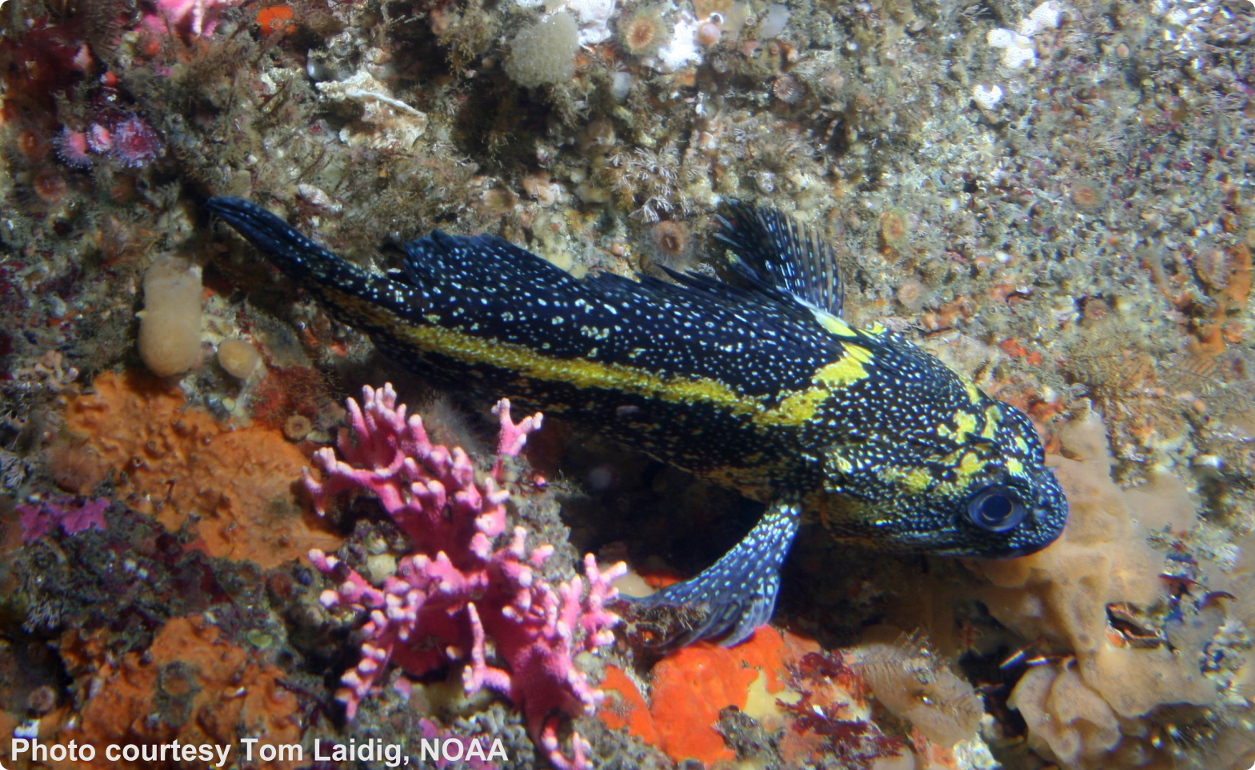
\includegraphics{cover_photo}~\\[1cm]
\pdftooltip{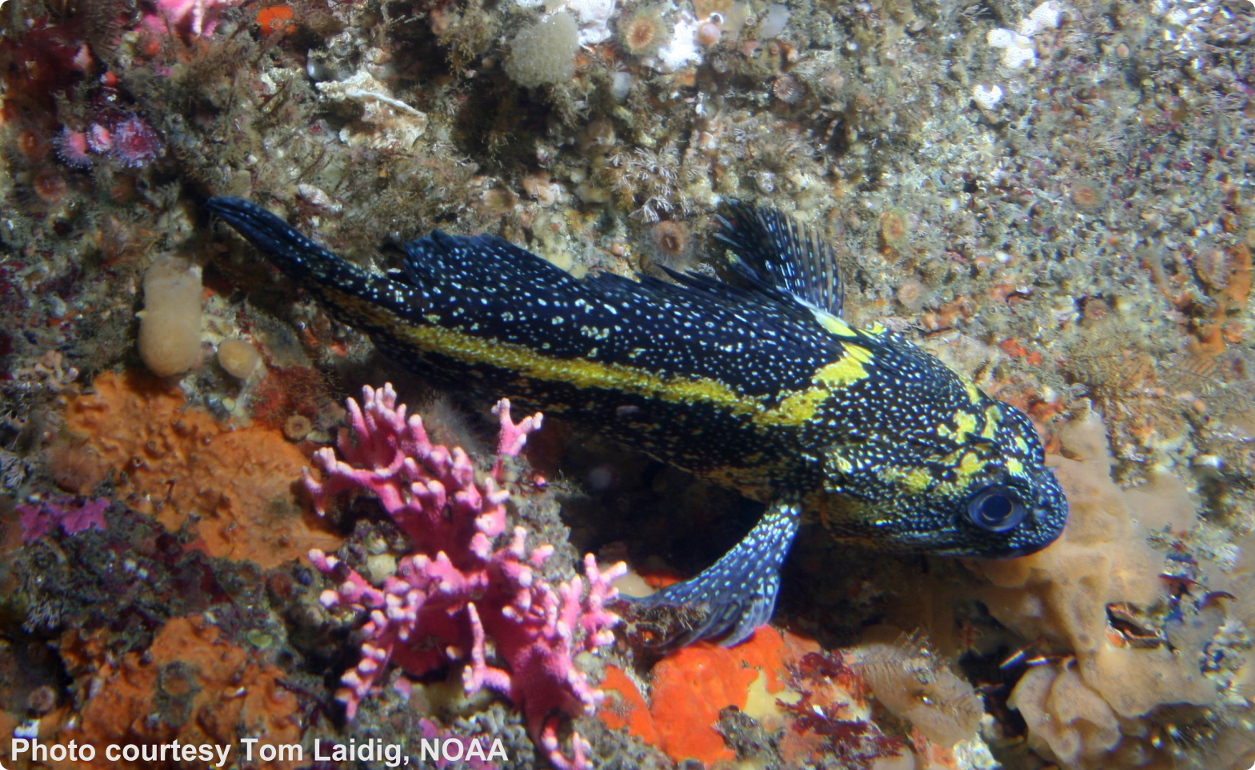
\includegraphics{cover_photo}}{This is a fish.}



Author No. 1\textsuperscript{1}\\
% Author No. 2\textsuperscript{2}\\
% Author No. 3\textsuperscript{3}\\

\vspace{.5cm}
% 
% \small
% \textsuperscript{1}Southwest Fisheries Science Center, U.S. Department of Commerce, National Oceanic and Atmospheric Administration, National Marine Fisheries Service, 110 Shaffer Road, Santa Cruz, California 95060\\

\vspace{.3cm}

\textsuperscript{1}Northwest Fisheries Science Center, U.S. Department of Commerce, National Oceanic and Atmospheric Administration, National Marine Fisheries Service, 2725 Montlake Boulevard East, Seattle, Washington 98112\\

\vspace{.3cm}

% \textsuperscript{3}Washington Department of Fish and Wildlife, 600 Capitol Way North, Olympia, Washington 98501\\


\vspace{.5cm}

\vfill
DRAFT SAFE\\
Disclaimer: This information is distributed solely for the purpose of pre-dissemination
peer review under applicable information quality guidelines. It has not been formally
disseminated by NOAA Fisheries. It does not represent and should not be construed to
represent any agency determination or policy. 

\vspace{.3cm}
%Bottom of the page
%{\large \today}


\newpage{\thispagestyle{empty}}


% \begin{flushleft}
% This report may be cited as:
% 
% ex. Monk, M. H. ,He, X., and Budrick, J. 2017. Status of the California Scorpionfish (\emph{Scorpaena guttata}) Off Southern California in 2017. Pacific Fishery Management Council, Portland, OR. Available from http://www.pcouncil.org/groundfish/stock-assessments/
% \end{flushleft}

\maketitle

\pagenumbering{roman}
\setcounter{page}{1}
\end{center}

{
\setcounter{tocdepth}{4}
\tableofcontents
}
\begin{verbatim}
## N models 3 
## Got three
\end{verbatim}

\begin{verbatim}
## Got 1
## Got 2
## End 2
## Got 3
\end{verbatim}

\setlength{\parskip}{5mm plus1mm minus1mm} \pagebreak

\setcounter{page}{1} \renewcommand{\thefigure}{\alph{figure}}
\renewcommand{\thetable}{\alph{table}}

\section*{Introduction}\label{introduction}
\addcontentsline{toc}{section}{Introduction}

\subsection*{Stock}\label{stock}
\addcontentsline{toc}{subsection}{Stock}

This assessment reports the status of the Black Rockfish
(\emph{Sebastes melanops}) resource in U.S. waters off the West Coast
using data through 2014, updated with catches through 2018 and with
projected catches for 2019 and 2020.

The models described in this document apply to the black rockfish
(Sebastes melanops) stocks that reside in the waters from Point
Conception (34°27' N latitude) in the south to the U.S. boundary with
Canada (approximately 48°30' N latitude). Following the consensus
recommendations from a preliminary stock assessment workshop in April
2015 (PFMC 2015), the stock assessment team (STAT) decided to prepare
separate geographic stock assessments that are spatially stratified with
boundaries at the CA/OR border (42°00' N latitude) and OR/WA border
(46°16' N latitude).

Black rockfish are also caught from the waters off British Columbia and
Alaska, but there have not been any formal assessments of stock status
for those areas.

\subsection*{Catches}\label{catches}
\addcontentsline{toc}{subsection}{Catches}

Information on historical landings of Black Rockfish are available back
to xxxx\ldots{} (Table \ref{tab:Exec_catch}). Commercial landings were
small during the years of World War II, ranging between 26 to 758 metric
tons (mt) per year.

Black rockfish are caught by a wide variety of gear types and in recent
decades have been a very important target species for recreational
charter-boats and private sport anglers in Washington and Oregon, and to
a lesser extent in California. In recent years the recreational fishery
has accounted for most of the black rockfish catches (Figure ES-1 to
Figure ES-3). Black rockfish can also be an important component of
nearshore commercial fisheries, either as incidental catch by the troll
fishery for salmon or as directed catch by jig fisheries for groundfish.
Further, in California and Oregon there are nearshore fisheries that
catch and sell fish live for the restaurant trade. Washington closed
nearshore commercial fisheries in state water in late 1990's and never
allowed the live-fish fishery to develop. In all states there have been
almost no trawl-caught landings of black rockfish in recent years (Table
ES-1), but trawl landings in the past were substantial (Figure ES-1 to
Figure ES-3).

Detailed reports of commercial landings of black rockfish are generally
unavailable prior to 1981, when the Pacific Fishery Information Network
(PacFIN) database began. The catch series prior to 1981 for these
assessments were derived by applying available estimates or assumed
values for the proportion of black rockfish landings in reported
landings of rockfish. Observer data, which are available only for the
past decade, indicate low levels of discarding of black rockfish,
generally less than 2\% of total catch. Because of their nearshore
distribution and low abundance compared to other rockfish species, black
rockfish are unlikely to have ever comprised a large percentage of
rockfish landings, but it seems quite certain that they have been more
than a trivial component for many years. Black rockfish were one of only
four rockfish species mentioned by scientific name in reports of
rockfish landings in Oregon during the 1940s, and they were one of only
six rockfish species mentioned by scientific name in reports of rockfish
landings in California during the same period. Mentions of black
rockfish extend back before the year 1900 in Washington.

(Figures \ref{fig:Exec_catch1}-\ref{fig:Exec_catch2})\\
(Figure \ref{fig:r4ss_catches})

Since 2000, annual total landings of Black Rockfish have ranged between
188-356 mt, with landings in 2014 totaling 356 mt.

\subsection*{Data and Assessment}\label{data-and-assessment}
\addcontentsline{toc}{subsection}{Data and Assessment}

This is a catch-only update of the assessment conducted in 2015. The
assessment assumes three areas delineated by state borders, as was
agreed upon at a pre-assessment and data workshop in March 2015. The
current assessment use the same versions of Stock Synthesis 3 as in
2015. The Washington base-case assessment includes two commercial and a
single recreational fleet, and a dockside and tag-based CPUE series. The
Oregon assessment has three commercial fleets and two recreational
fleets, and uses five surveys and an additional research study for
biological compositions. California also has three commercial fleets and
1 recreational fleet with three surveys of abundance, all based on
recreational fisheries. All three models include length compositions,
and conditional age-at-length data.

\subsubsection*{Sigma analysis}\label{sigma-analysis}
\addcontentsline{toc}{subsubsection}{Sigma analysis}

One purpose of this assessment is to evaluate the effect of increasing
the sigma value used to calculate P* buffers as the assessment ages, and
the three models were each run with a series of buffers calculated from
an increasing sigma. The Washington and California stocks are Category I
stocks, and the models used buffers calculated from the 0.45 value of
sigma. For the Oregon model, these were calculated according to the
default Category II values. The timeseries of catches, projections and
buffers used for this analysis were all provided by the Groundfish
Management Team (GMT) of the Pacific Fishery Management Council (PFMC).

\subsection*{Ecosystem Considerations}\label{ecosystem-considerations}
\addcontentsline{toc}{subsection}{Ecosystem Considerations}

Ecosystem considerations were not explicitly explored in these models,
though growth deviations were considered in the Washington model. While
no mechanisms have been put forth for these time-varying changes in
growth, an environmental component is possible. Limited data in Oregon
and California also suggest the possibility that growth has changed over
time.

\subsection*{Unresolved Problems and Major
Uncertainties}\label{unresolved-problems-and-major-uncertainties}
\addcontentsline{toc}{subsection}{Unresolved Problems and Major
Uncertainties}

The most significant uncertainty for all models is the treatment and
value of natural mortality and the form of fleet selectivity (e.g.,
length-based asymptotic vs.~age-based dome-shaped selectivity).
Data-driven selection between the extreme ``kill'' (using a ramping of
M) or ``hide'' hypotheses are not currently resolvable. The current
California and Washington base models instead use a form of the ``kill''
hypothesis by not implementing the age-based selectivity (``hide''
hypothesis) and estimating female and male natural mortality, thus
avoiding a fixing natural mortality as was necessary in the Oregon
model.

The Oregon model also contained a step in female natural mortality, a
specification not used in the California or Washington models. Another
important issue is the highly uncertain historical time-series of
removals in all states, which needs further consideration.

The development of fishery-dependent indices of abundance still requires
further attention. Steepness, while fixed, is still highly uncertain for
rockfishes and currently is mismatched to the MSY proxy. And while the
steepness profile shows low sensitivity in several derived quantities,
steepness strongly defines the yield capacity of stocks, and therefore
could cause major uncertainty in the recommended management quantities.
Stock structure and its relationship to the current political/management
boundaries are also not fully understood, both within U.S. jurisdiction
and between the U.S. and Canada. While this is a common challenge faced
in most west coast stock assessments, further improvement on this issue
will likely rely on black rockfish-specific data.

\subsection*{Research and Data Needs}\label{research-and-data-needs}
\addcontentsline{toc}{subsection}{Research and Data Needs}

Recommended avenues for research to help improve future black rockfish
stock assessments:

\begin{enumerate}

\item \textbf{Movement}: Further investigation into the movement and behavior of older (> age 10) females to reconcile their absence in fisheries data. If the females are currently inaccessible to fishing gear, can we determine where they are?

\item \textbf{Mortality}: Appropriate natural mortality values for females and males will help resolve the extent to which dome-shaped age-based selectivity may be occurring for each.

\item \textbf{Historical Catch}:  All states need improved historical catch reconstructions. The trawl fishery catches in particular require attention. Given the huge historical removals of that fleet in each state, the assessment is very sensitive to the assumed functional form of selectivity. A synoptic catch reconstruction is recommended, where states work together to resolve cross-border catch issues as well as standardize the approach to catch recommendations.

\item \textbf{Uncertainty}: Identifying stanzas or periods of uncertainty in the historical catch series will aid in the exploration of catch uncertainty in future assessment sensitivity runs.

\item \textbf{Habitat}: The ODFW tagging study off Newport should continue and be expanded to other areas. To provide better prior information on the spatial distribution of the black rockfish stock, further work should be conducted to map the extent of black rockfish habitat and the densities of black rockfish residing there.

\item \textbf{Survey}:  An independent nearshore survey should be supported in all states to avoid the reliance on fishery-based CPUE indices.

\item \textbf{Stock Structure}:  Stock structure for black rockfish is a complicated topic that calls for further analysis. How this is determined (e.g., exploitation history, genetics, life history variability, biogeography, etc.) and what this means for management units needs to be further refined. This is a general issue for all nearshore stocks that likely have significant and small scale stock structure among and within states, but limited data collections to support small-scale management.

\end{enumerate}

\section*{Executive summary for the California
Model}\label{executive-summary-for-the-california-model}
\addcontentsline{toc}{section}{Executive summary for the California
Model}

\FloatBarrier

\begin{figure}[htbp]
\centering
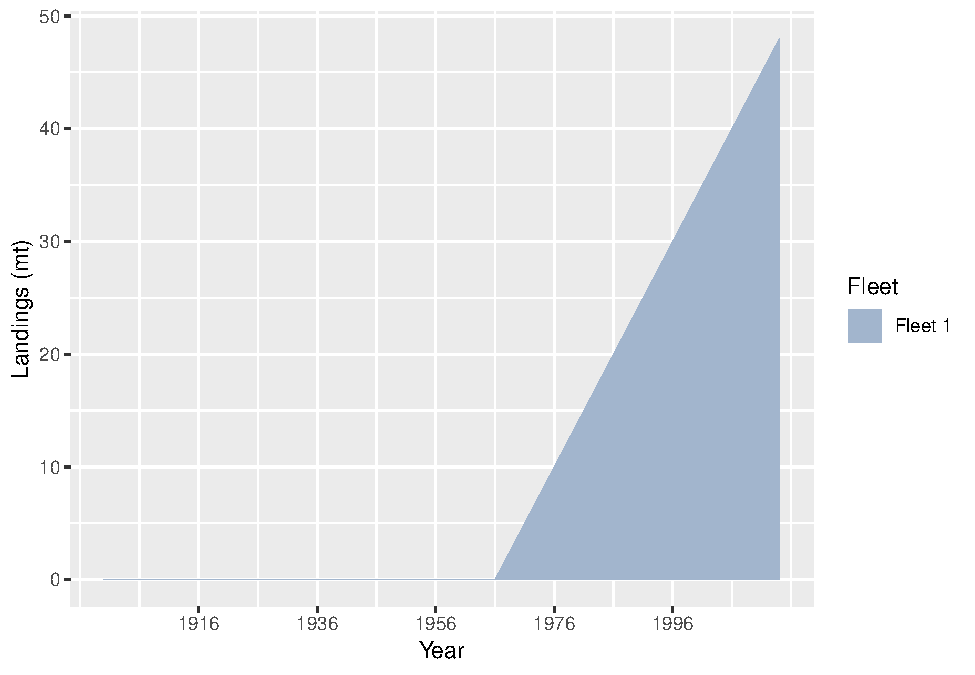
\includegraphics{00_Assessment_Compile_files/figure-latex/unnamed-chunk-4-1.pdf}
\caption{Black Rockfish catch history for the CA recreational fleets.
\label{fig:Exec_catch1}}
\end{figure}

\FloatBarrier

\begin{figure}[htbp]
\centering
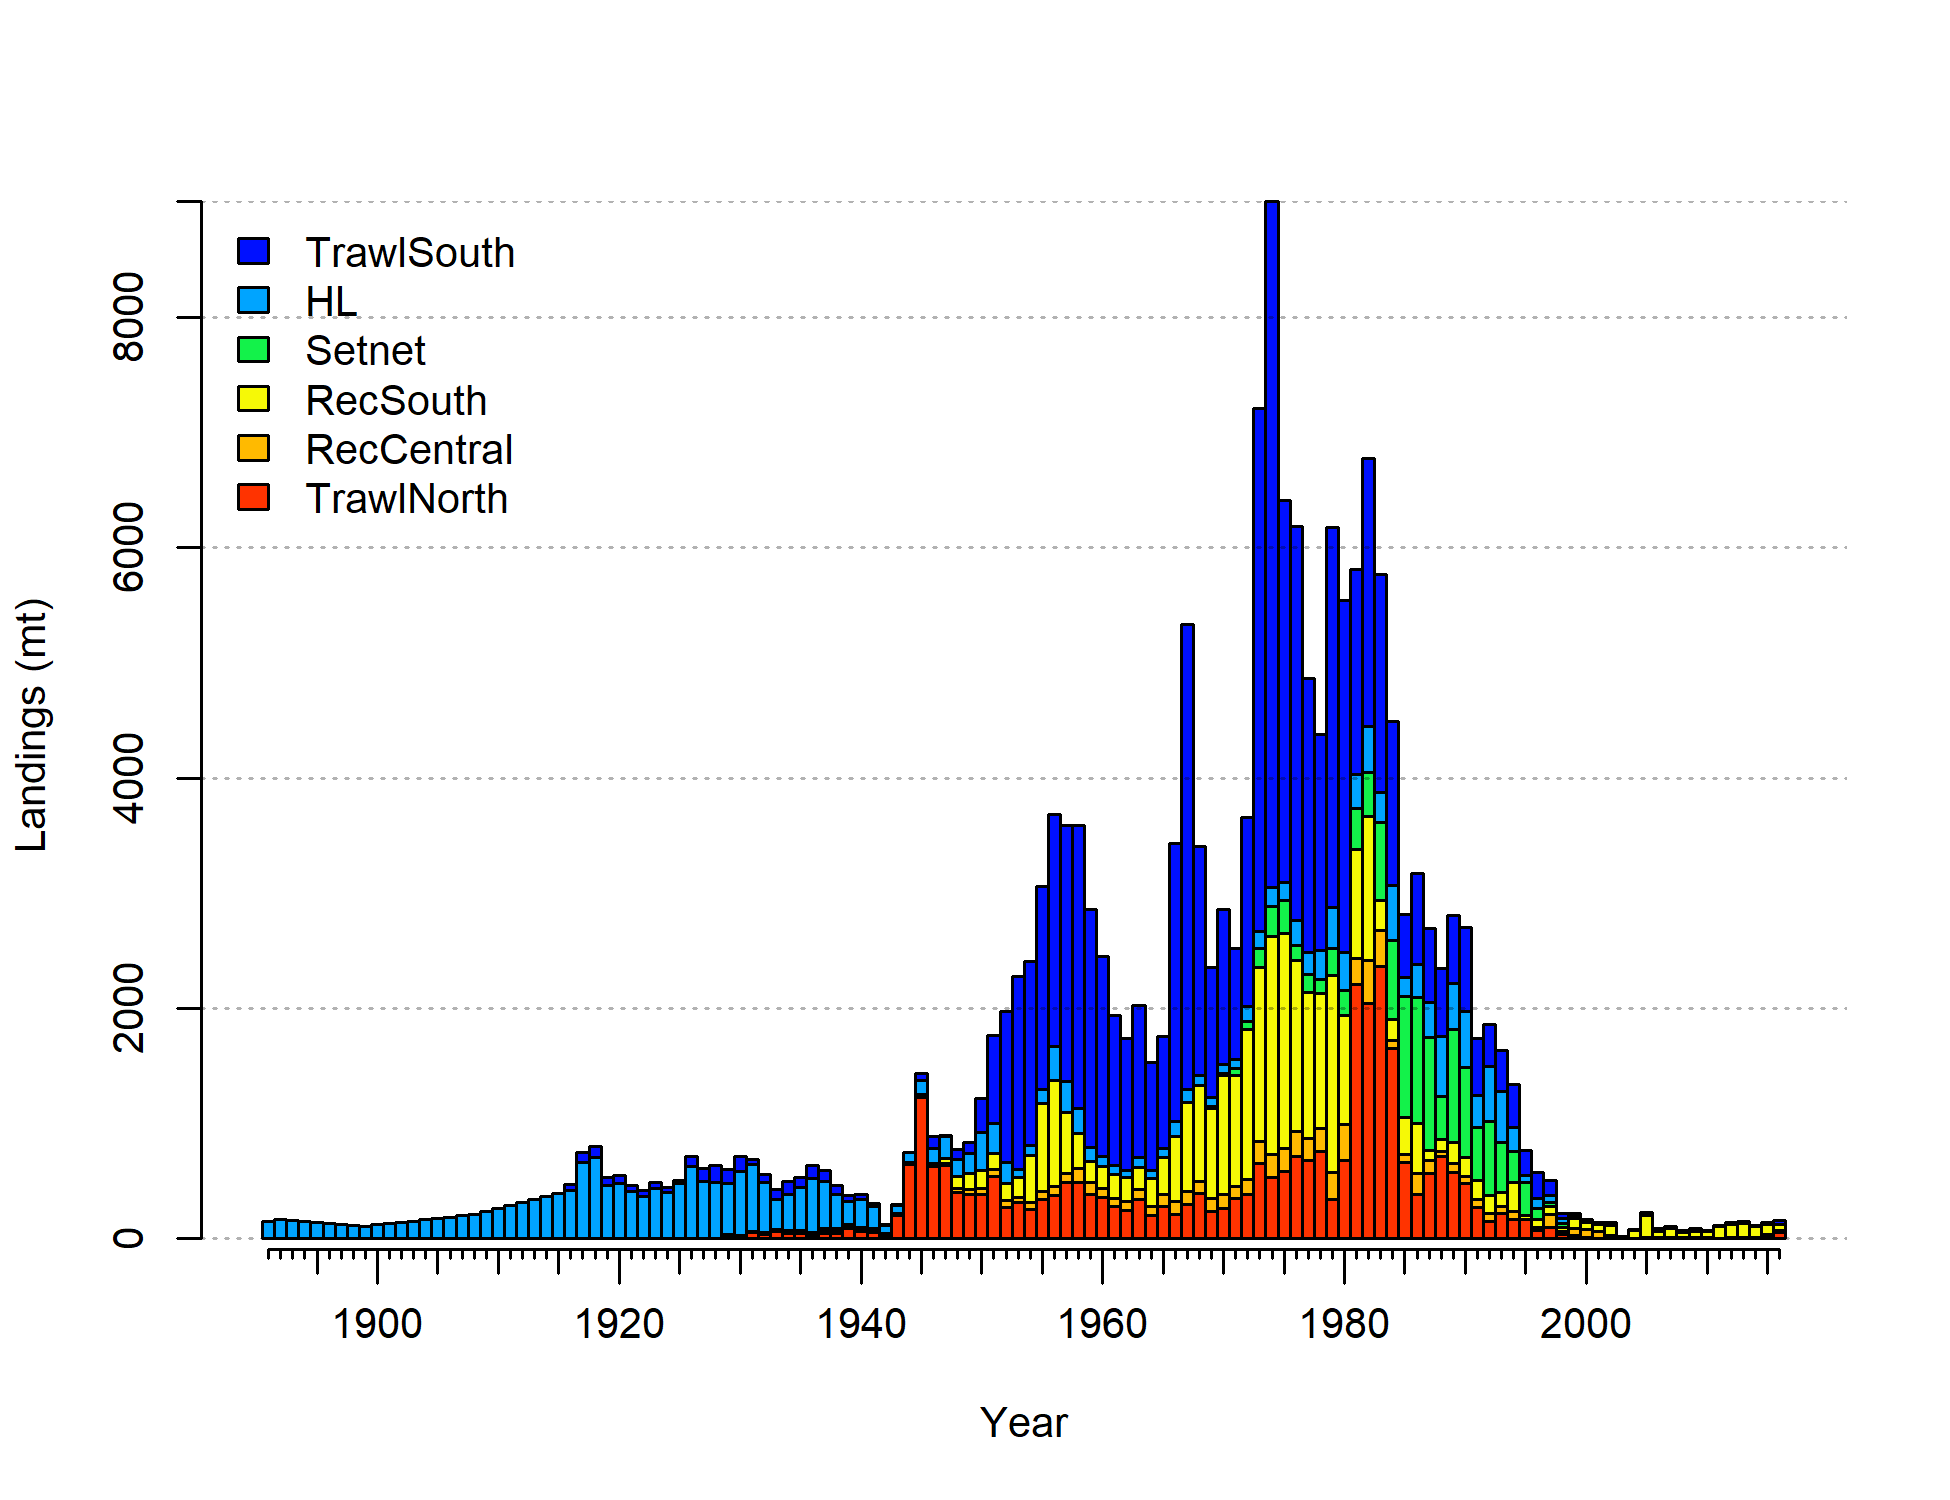
\includegraphics{r4ss/plots_mod1/catch2 landings stacked.png}
\caption{Catch history of Black Rockfish in the California model.
\label{fig:r4ss_catches}}
\end{figure}

\begin{table}[ht]
\centering
\caption{Recent Black Rockfish landings (mt) by 
                                            fleet.} 
\label{tab:Exec_catch}
\begin{tabular}{l>{\centering}p{1in}>{\centering}p{1in}>{\centering}p{1in}>{\centering}p{.9in}>{\centering}p{.9in}>{\centering}p{.6in}}
  \hline
Year & Landings 1 & Landings 2 & Landings 3 & Landings 4 & Landings 5 & Total \\ 
  \hline
2005 & - & - & - & - & - & - \\ 
  2006 & - & - & - & - & - & - \\ 
  2007 & - & - & - & - & - & - \\ 
  2008 & - & - & - & - & - & - \\ 
  2009 & - & - & - & - & - & - \\ 
  2010 & - & - & - & - & - & - \\ 
  2011 & - & - & - & - & - & - \\ 
  2012 & - & - & - & - & - & - \\ 
  2013 & - & - & - & - & - & - \\ 
  2014 & - & - & - & - & - & - \\ 
   \hline
\end{tabular}
\end{table}

\FloatBarrier

\newpage

\FloatBarrier

\subsection*{Stock Biomass}\label{stock-biomass}
\addcontentsline{toc}{subsection}{Stock Biomass}

(Figure \ref{fig:Spawnbio_all} and Table
\ref{tab:SpawningDeplete_mod1}).

The 2014 estimated spawning biomass relative to unfished equilibrium
spawning biomass is above the target of 40\% of unfished spawning
biomass at 33.3\% (95\% asymptotic interval: \(\pm\) 18.9\%-47.7\%)
(Figure \ref{fig:RelDeplete_all}). Approximate confidence intervals
based on the asymptotic variance estimates show that the uncertainty in
the estimated spawning biomass is high.

\FloatBarrier

\begin{table}[ht]
\centering
\caption{Recent trend in beginning of the 
                                      year spawning output and depletion for
                                      the California model for Black Rockfish.} 
\label{tab:SpawningDeplete_mod1}
\begin{tabular}{l>{\centering}p{1.3in}>{\centering}p{1.2in}>{\centering}p{1in}>{\centering}p{1.2in}}
  \hline
Year & Spawning Output (million eggs) & \~{} 95\% confidence interval & Estimated depletion & \~{} 95\% confidence interval \\ 
  \hline
2006 & 227.850 & (144.7-311) & 0.215 & (0.129-0.3) \\ 
  2007 & 231.368 & (145.32-317.41) & 0.218 & (0.131-0.305) \\ 
  2008 & 241.187 & (150.58-331.79) & 0.227 & (0.136-0.318) \\ 
  2009 & 256.821 & (159.31-354.33) & 0.242 & (0.145-0.339) \\ 
  2010 & 267.775 & (161.81-373.74) & 0.252 & (0.147-0.357) \\ 
  2011 & 285.105 & (169.54-400.67) & 0.269 & (0.155-0.383) \\ 
  2012 & 305.208 & (180.43-429.98) & 0.288 & (0.165-0.41) \\ 
  2013 & 321.621 & (189.4-453.84) & 0.303 & (0.174-0.431) \\ 
  2014 & 329.401 & (190.94-467.86) & 0.310 & (0.177-0.444) \\ 
  2015 & 353.216 & (203.75-502.69) & 0.333 & (0.189-0.477) \\ 
   \hline
\end{tabular}
\end{table}

\FloatBarrier

\begin{figure}[htbp]
\centering
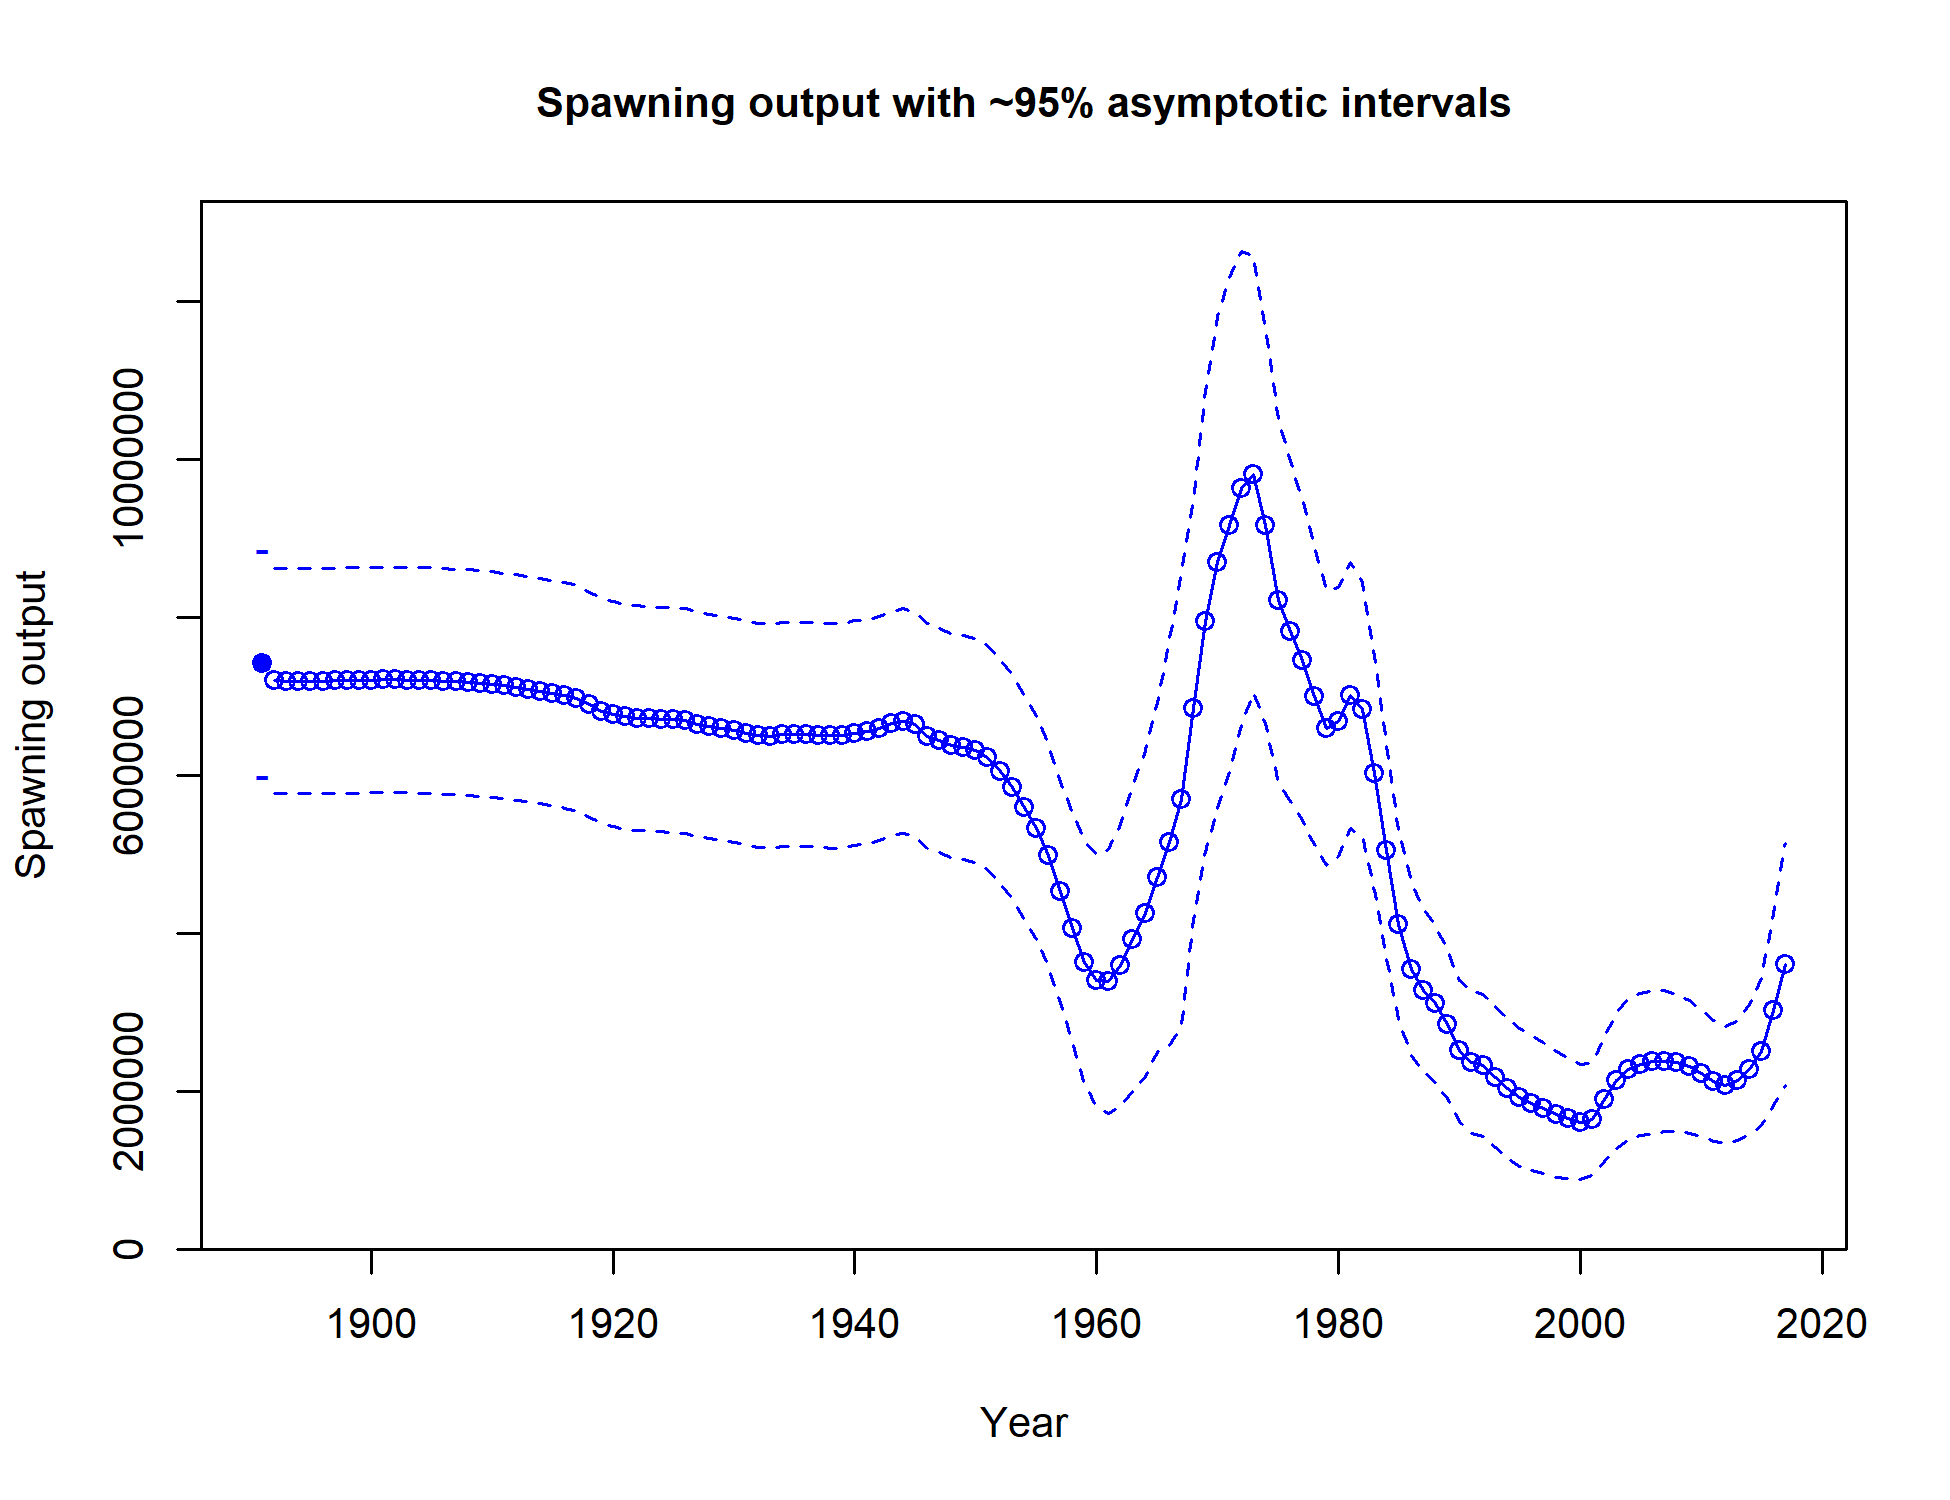
\includegraphics{r4ss/plots_mod1/ts7_Spawning_output_with_95_asymptotic_intervals_intervals.png}
\caption{Time series of spawning biomass trajectory (circles and line:
median; light broken lines: 95\% credibility intervals) for the base
case assessment model. \label{fig:Spawnbio_all}}
\end{figure}

\begin{figure}[htbp]
\centering
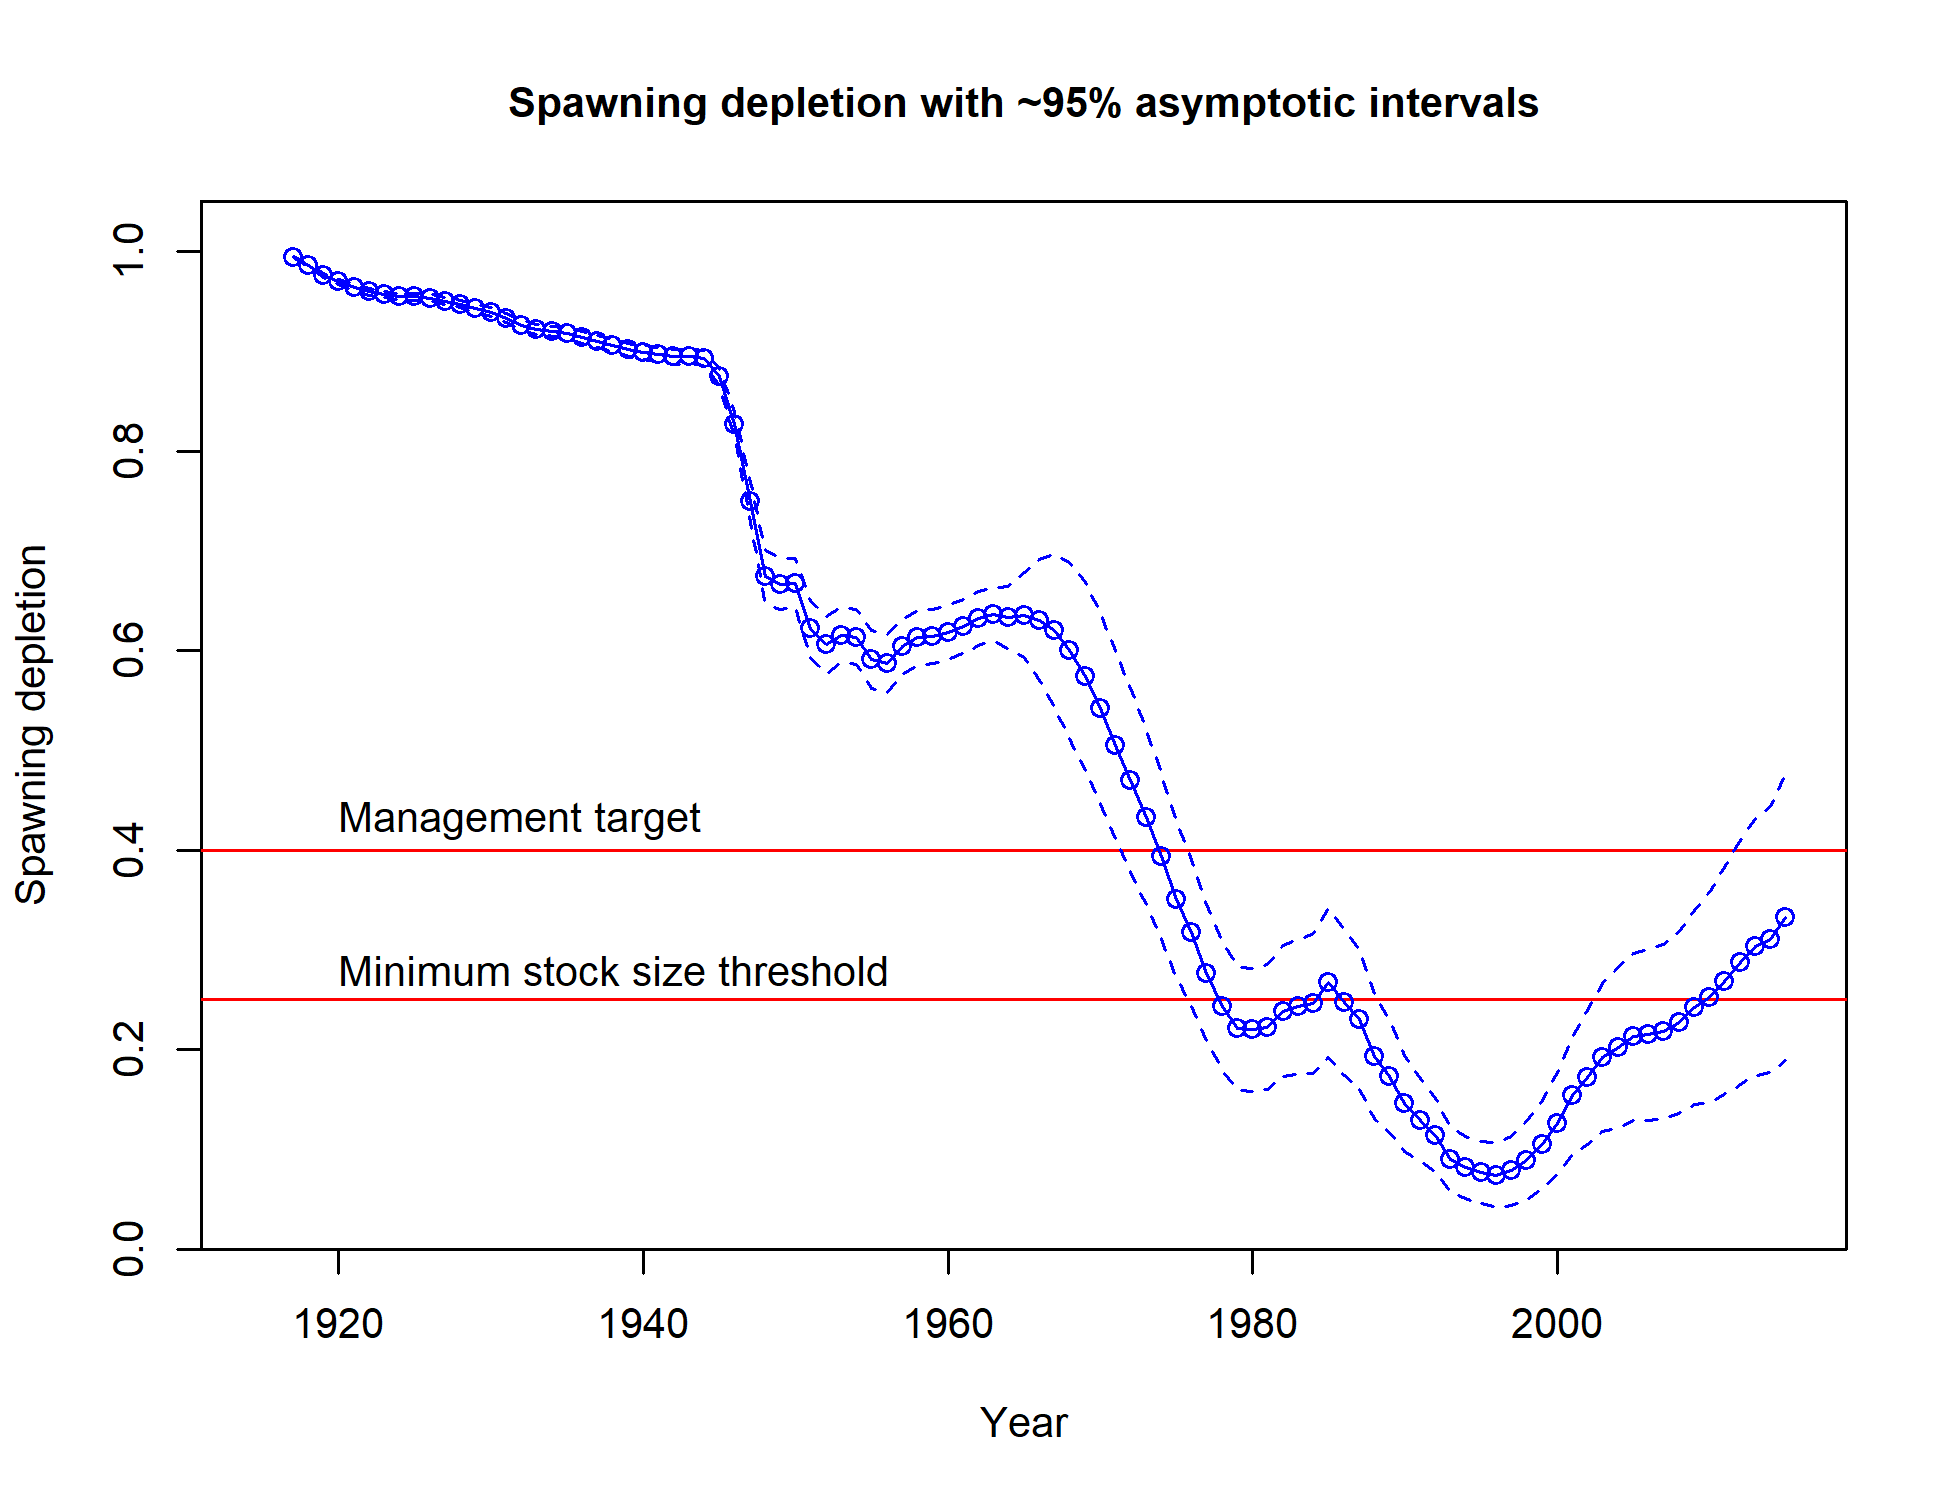
\includegraphics{r4ss/plots_mod1/ts9_Spawning_depletion_with_95_asymptotic_intervals_intervals.png}
\caption{Estimated relative depletion with approximate 95\% asymptotic
confidence intervals (dashed lines) for the base case assessment model.
\label{fig:RelDeplete_all}}
\end{figure}

\FloatBarrier

\subsection*{Recruitment}\label{recruitment}
\addcontentsline{toc}{subsection}{Recruitment}

Recruitment deviations were estimated from xxxx-xxxx (Figure
\ref{fig:Recruits_all} and Table \ref{tab:Recruit_mod1}).

\begin{table}[ht]
\centering
\caption{Recent recruitment for the California model.} 
\label{tab:Recruit_mod1}
\begin{tabular}{>{\centering}p{.8in}>{\centering}p{1.6in}>{\centering}p{1.3in}}
  \hline
Year & Estimated Recruitment (1,000s) & \~{} 95\% confidence interval \\ 
  \hline
2006 & 984.26 & (585.85 - 1653.62) \\ 
  2007 & 1326.80 & (756.15 - 2328.1) \\ 
  2008 & 4508.71 & (2710.76 - 7499.17) \\ 
  2009 & 4323.29 & (2318.79 - 8060.6) \\ 
  2010 & 2997.05 & (1493.29 - 6015.09) \\ 
  2011 & 1764.55 & (798.38 - 3899.95) \\ 
  2012 & 1700.52 & (1273.7 - 2270.38) \\ 
  2013 & 1719.46 & (1292.47 - 2287.52) \\ 
  2014 & 1727.92 & (1299.38 - 2297.79) \\ 
  2015 & 1751.93 & (1322.75 - 2320.36) \\ 
   \hline
\end{tabular}
\end{table}

\FloatBarrier

\begin{figure}[htbp]
\centering
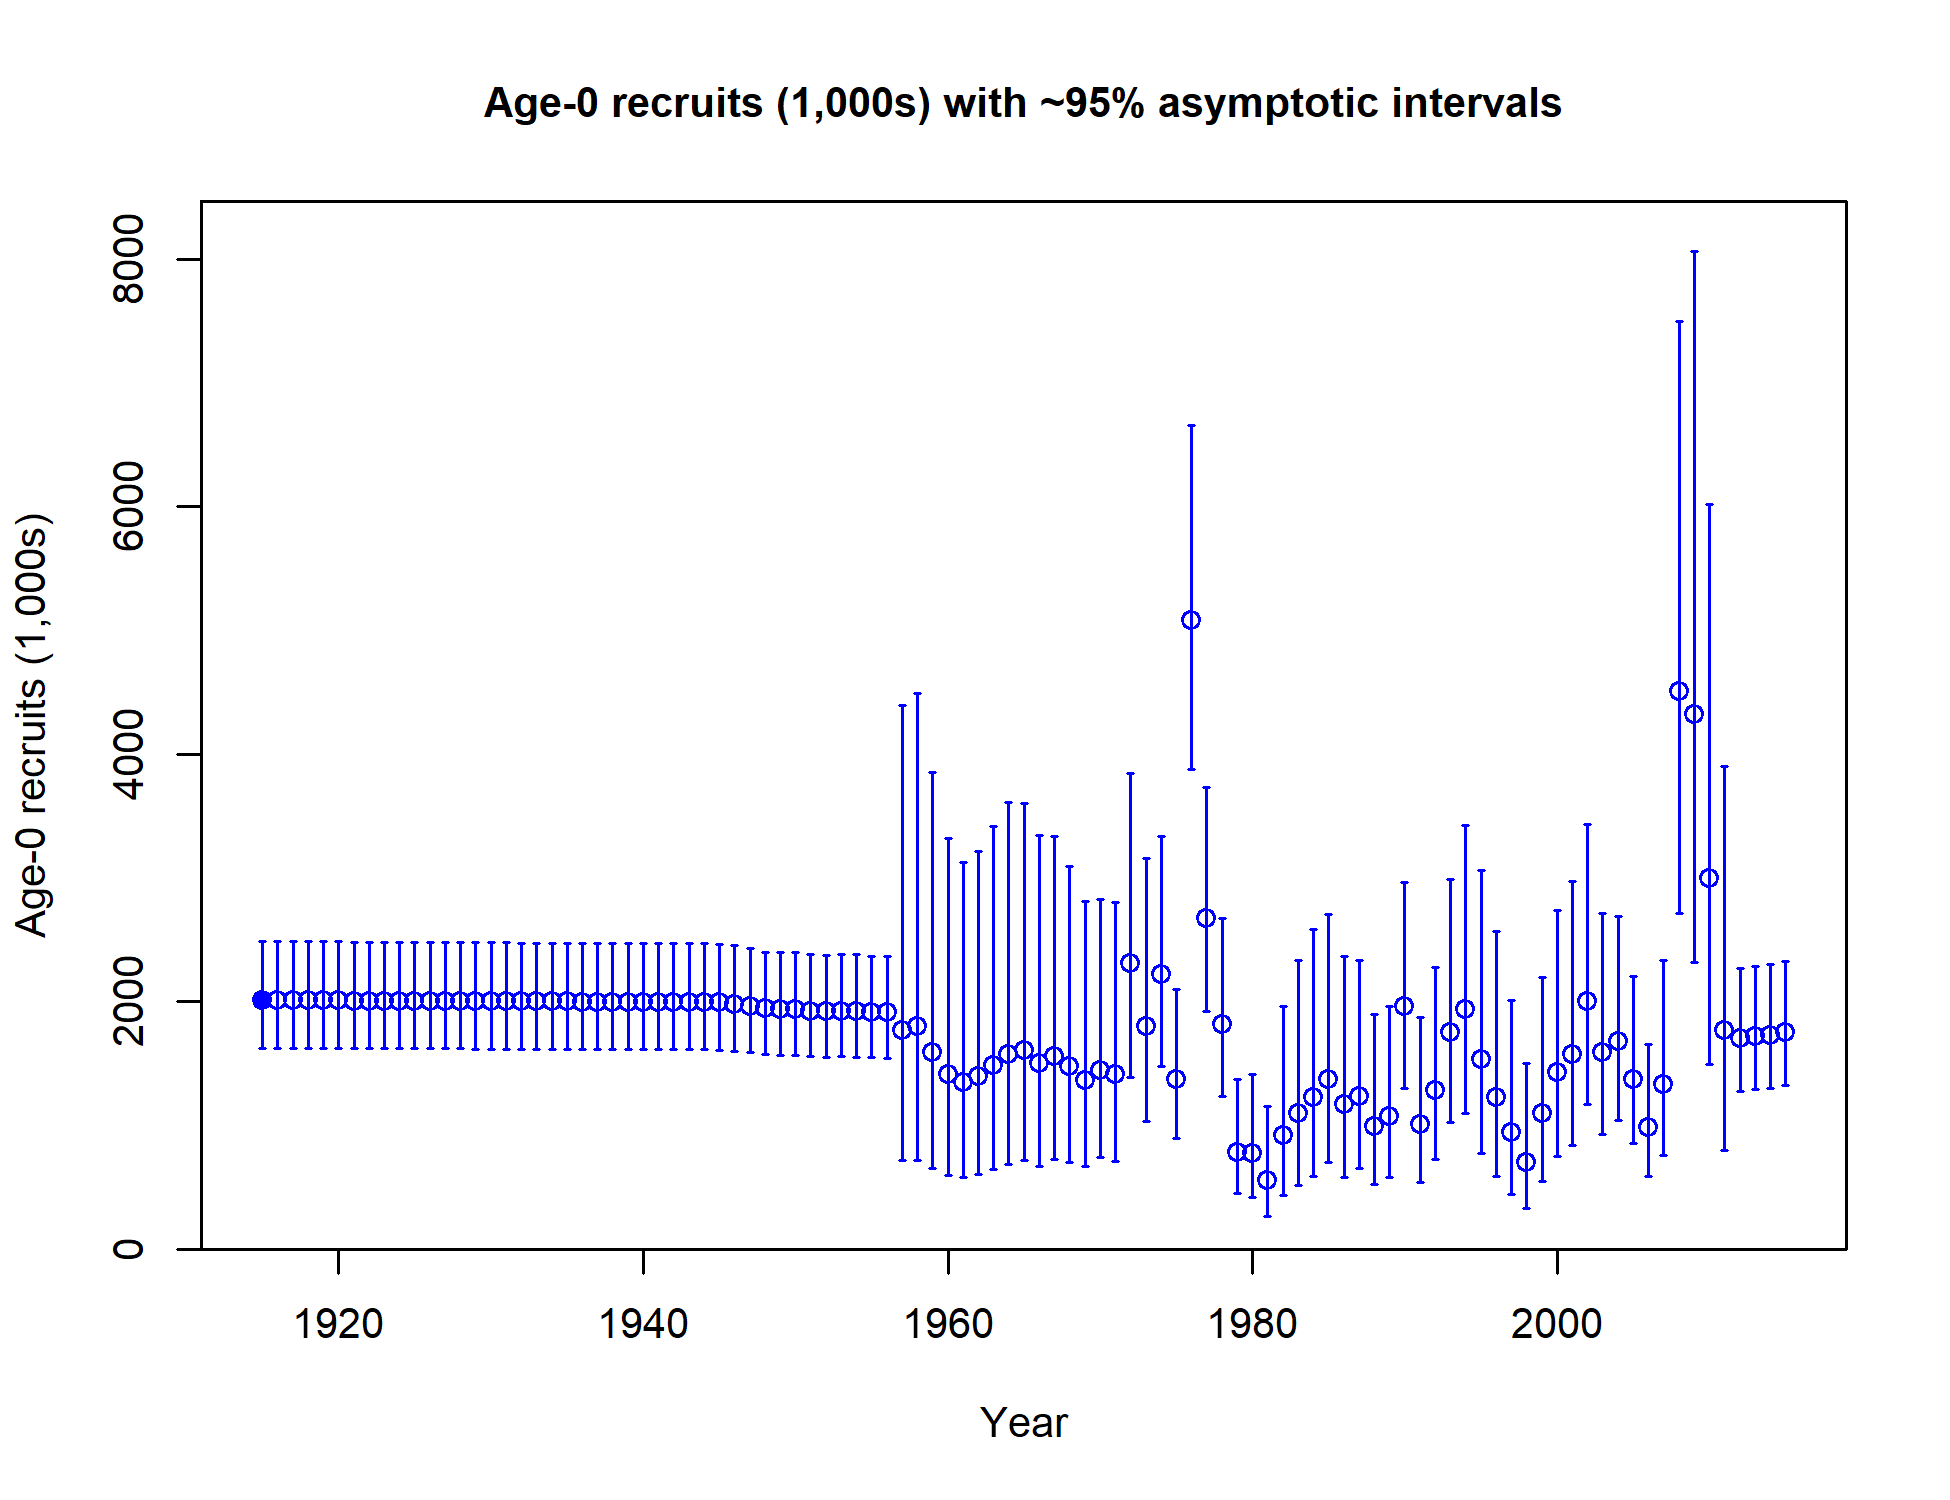
\includegraphics{r4ss/plots_mod1/ts11_Age-0_recruits_(1000s)_with_95_asymptotic_intervals.png}
\caption{Time series of estimated Black Rockfish recruitments for the
base-case model with 95\% confidence or credibility intervals.
\label{fig:Recruits_all}}
\end{figure}

\FloatBarrier

\subsection*{Exploitation status}\label{exploitation-status}
\addcontentsline{toc}{subsection}{Exploitation status}

Harvest rates estimated by the base model \ldots{}.. management target
levels (Table \ref{tab:SPR_Exploit_mod1} and Figure \ref{fig:SPR_all}).

\FloatBarrier

\begin{table}[ht]
\centering
\caption{Recent trend in spawning potential 
                                        ratio and exploitation for Black Rockfish in the California model.  Fishing intensity is (1-SPR) 
                                        divided by 50\% (the SPR target) and exploitation 
                                        is F divided by F\textsubscript{SPR}.} 
\label{tab:SPR_Exploit_mod1}
\begin{tabular}{l>{\centering}p{1in}>{\centering}p{1.2in}>{\centering}p{1in}>{\centering}p{1.2in}}
  \hline
Year & Fishing intensity & \~{} 95\% confidence interval & Exploitation rate & \~{} 95\% confidence interval \\ 
  \hline
2005 & 1.20 & (0.96-1.44) & 0.09 & (0.06-0.12) \\ 
  2006 & 1.15 & (0.91-1.4) & 0.08 & (0.06-0.11) \\ 
  2007 & 1.06 & (0.81-1.31) & 0.08 & (0.05-0.1) \\ 
  2008 & 1.06 & (0.81-1.31) & 0.08 & (0.05-0.1) \\ 
  2009 & 1.30 & (1.04-1.55) & 0.10 & (0.07-0.14) \\ 
  2010 & 1.12 & (0.85-1.38) & 0.08 & (0.05-0.11) \\ 
  2011 & 0.92 & (0.67-1.18) & 0.06 & (0.04-0.08) \\ 
  2012 & 0.89 & (0.65-1.14) & 0.05 & (0.03-0.07) \\ 
  2013 & 1.14 & (0.88-1.41) & 0.08 & (0.05-0.11) \\ 
  2014 & 1.07 & (0.8-1.33) & 0.07 & (0.05-0.1) \\ 
   \hline
\end{tabular}
\end{table}

\FloatBarrier

\begin{figure}[htbp]
\centering
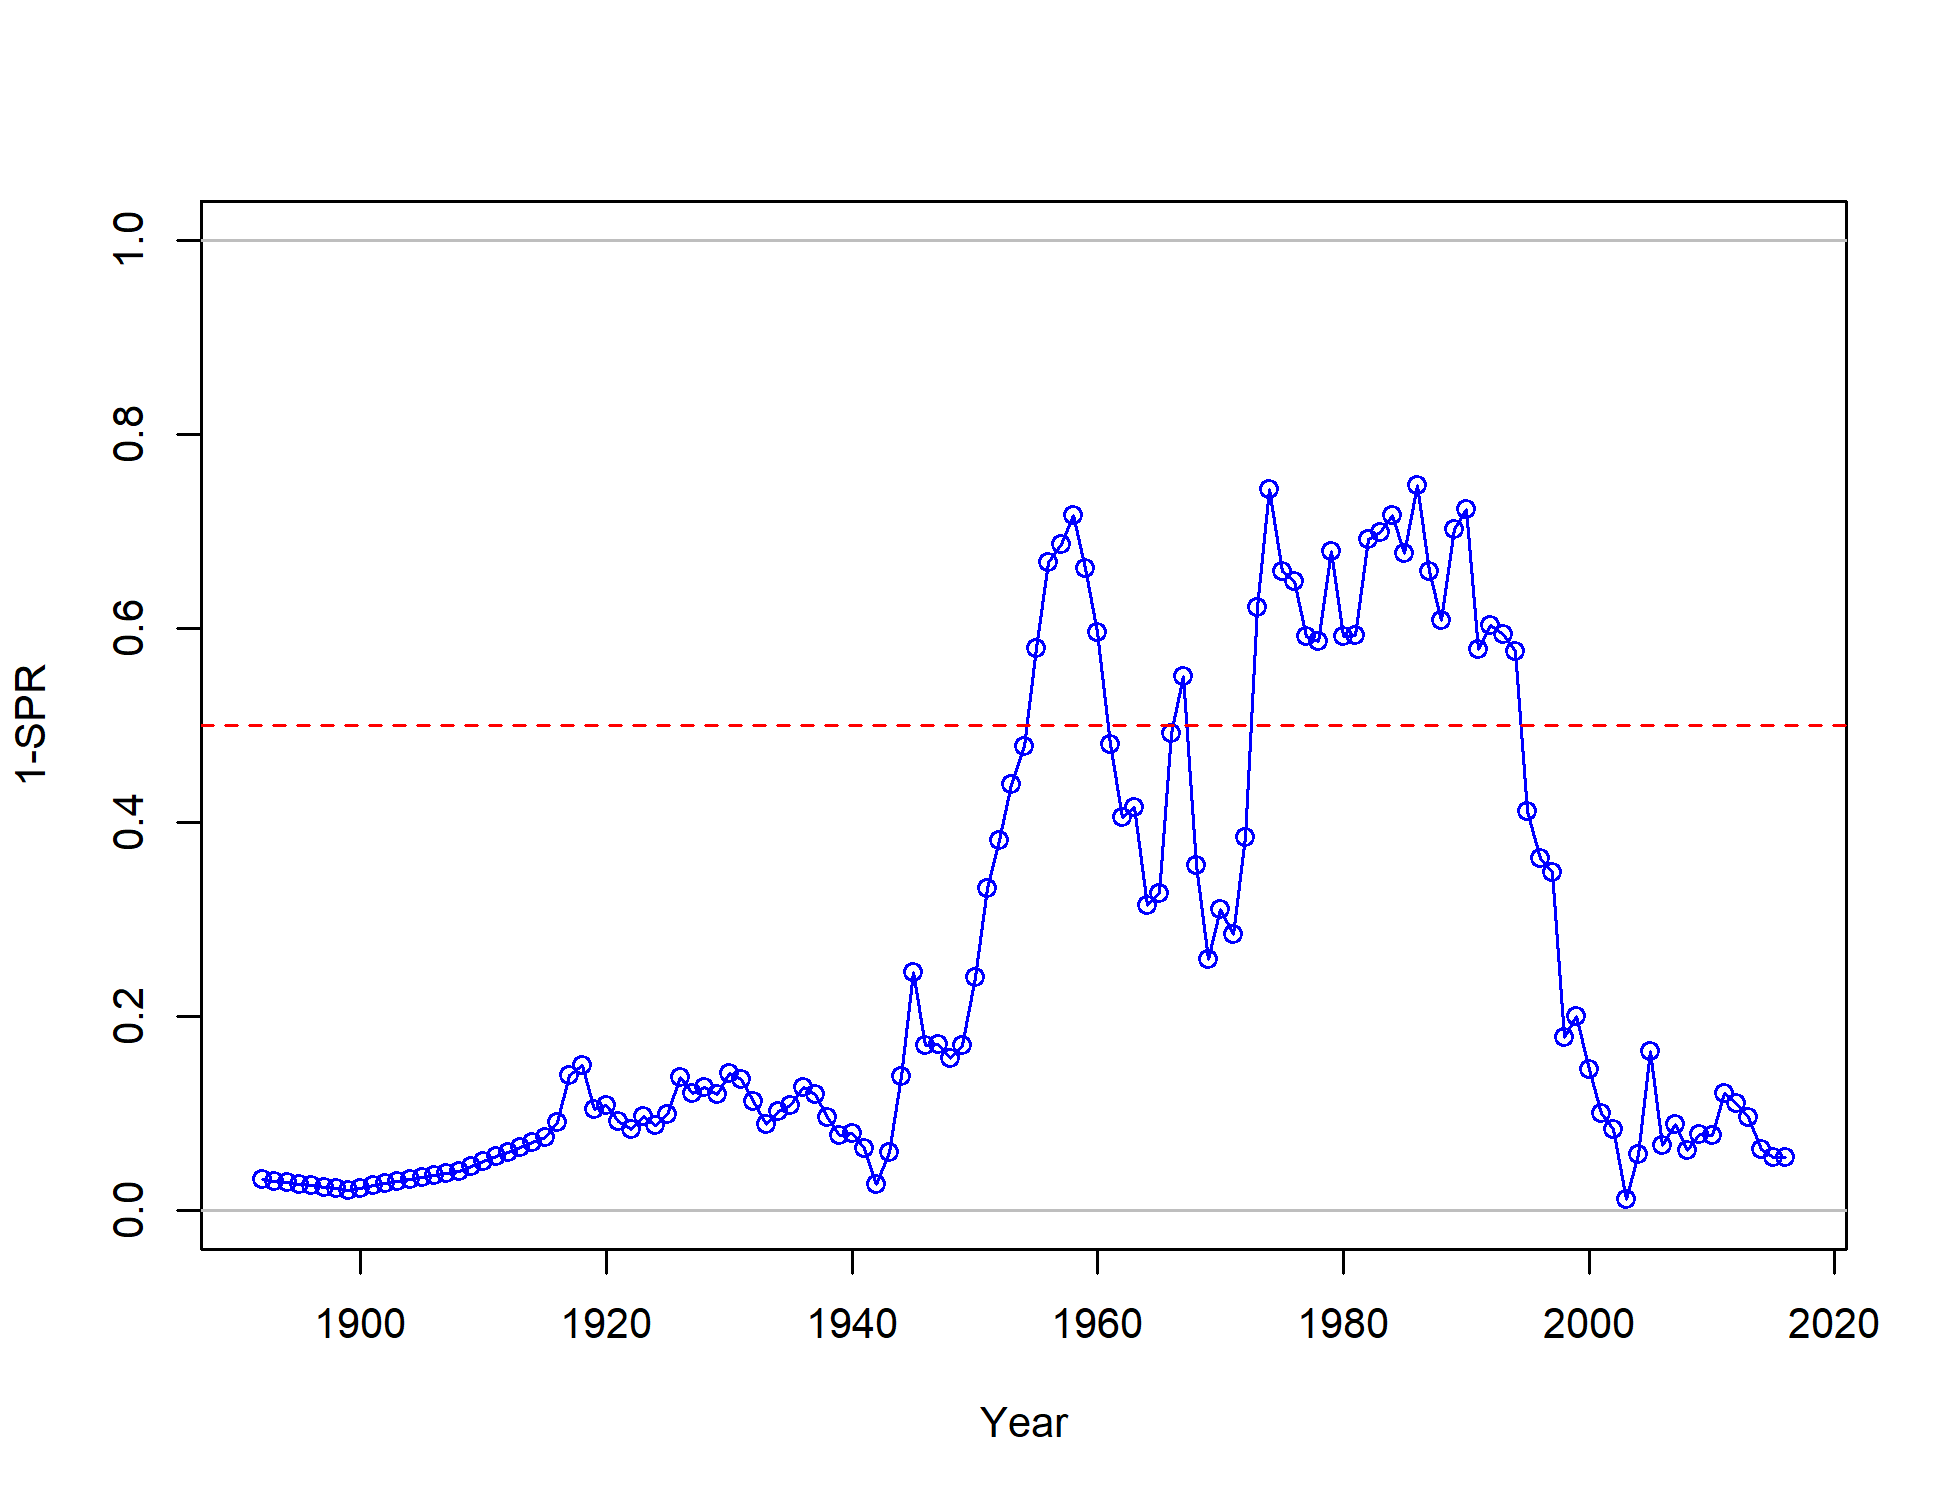
\includegraphics{r4ss/plots_mod1/SPR2_minusSPRseries.png}
\caption{Estimated spawning potential ratio (SPR) for the base-case
model. One minus SPR is plotted so that higher exploitation rates occur
on the upper portion of the y-axis. The management target is plotted as
a red horizontal line and values above this reflect harvests in excess
of the overfishing proxy based on the SPR\textsubscript{50\%} harvest
rate. The last year in the time series is 2014. \label{fig:SPR_all}}
\end{figure}

\FloatBarrier

\subsection*{Reference Points}\label{reference-points}
\addcontentsline{toc}{subsection}{Reference Points}

This stock assessment estimates that Black Rockfish in the California
model is below the biomass target (\(SB_{40\%}\)), and well above the
minimum stock size threshold (\(SB_{25\%}\)). The estimated relative
depletion level for the base model in 2015 is 33.3\% (95\% asymptotic
interval: \(\pm\) 18.9\%-47.7\%, corresponding to an unfished spawning
biomass of 353.216 million eggs (95\% asymptotic interval: 203.75-502.69
million eggs) of spawning biomass in the base model (Table
\ref{tab:Ref_pts_mod1}). Unfished age 1+ biomass was estimated to be
9,540 mt in the base case model. The target spawning biomass
(\(SB_{40\%}\)) is 425 million eggs, which corresponds with an
equilibrium yield of 343 mt. Equilibrium yield at the proxy \(F_{MSY}\)
harvest rate corresponding to \(SPR_{50\%}\) is 319 mt (Figure
\ref{fig:Yield_all}).

\FloatBarrier

\begin{table}[ht]
\centering
\caption{Summary of reference 
                                      points and management quantities for the 
                                      base case California model.} 
\label{tab:Ref_pts_mod1}
\begin{tabular}{>{\raggedright}p{4.1in}>{\raggedleft}p{.62in}>{\raggedleft}p{.62in}>{\raggedleft}p{.62in}}
  \hline
\textbf{Quantity} & \textbf{Estimate} & \textbf{Low 2.5\%  limit} & \textbf{High 2.5\%  limit} \\ 
  \hline
Unfished spawning output (million eggs) & 1,062 & 830 & 1,293 \\ 
  Unfished age 1+ biomass (mt) & 9,540 & 8,862 & 10,219 \\ 
  Unfished recruitment ($R_{0}$) & 2,010 & 1,580 & 2,440 \\ 
  Spawning output(2014 million eggs) & 329 & 191 & 468 \\ 
  Depletion (2014) & 0.31 & 0.177 & 0.444 \\ 
  \textbf{$\text{Reference points based on } \mathbf{SB_{40\%}}$} &  &  &  \\ 
  Proxy spawning output ($B_{40\%}$) & 425 & 332 & 517 \\ 
  SPR resulting in $B_{40\%}$ ($SPR_{B40\%}$) & 0.444 & 0.444 & 0.444 \\ 
  Exploitation rate resulting in $B_{40\%}$ & 0.075 & 0.07 & 0.081 \\ 
  Yield with $SPR_{B40\%}$ at $B_{40\%}$ (mt) & 343 & 316 & 369 \\ 
  \textbf{\textit{Reference points based on SPR proxy for MSY}} &  &  &  \\ 
  Spawning output & 489 & 382 & 595 \\ 
  $SPR_{proxy}$ & 0.5 &  &  \\ 
  Exploitation rate corresponding to $SPR_{proxy}$ & 0.064 & 0.059 & 0.069 \\ 
  Yield with $SPR_{proxy}$ at $SB_{SPR}$ (mt) & 319 & 295 & 344 \\ 
  \textbf{\textit{Reference points based on estimated MSY values}} &  &  &  \\ 
  Spawning output at $MSY$ ($SB_{MSY}$) & 254 & 199 & 309 \\ 
  $SPR_{MSY}$ & 0.295 & 0.287 & 0.303 \\ 
  Exploitation rate at $MSY$ & 0.117 & 0.107 & 0.126 \\ 
  $MSY$ (mt)  & 376 & 345 & 408 \\ 
   \hline
\end{tabular}
\end{table}

\FloatBarrier

\subsection*{Management Performance}\label{management-performance}
\addcontentsline{toc}{subsection}{Management Performance}

Table \ref{tab:mnmgt_perform}

\begin{table}[ht]
\centering
\caption{Recent trend in total catch and commercial 
                              landings (mt) relative to the management guidelines. 
                              Estimated total catch reflect the commercial landings 
                              plus the model estimated discarded biomass.} 
\label{tab:mnmgt_perform}
\scalebox{0.9}{
\begin{tabular}{>{\raggedleft}p{1in}>{\centering}p{1in}>{\centering}p{1in}>{\centering}p{1in}>{\centering}p{1in}}
  \hline
Year & OFL (mt; ABC prior to 2011) & ABC (mt) & ACL (mt; OY prior to 2011) & Estimated total catch (mt) \\ 
  \hline
\textbf{2007} & - & - & - & - \\ 
  \textbf{2008} & - & - & - & - \\ 
  \textbf{2009} & - & - & - & - \\ 
  \textbf{2010} & - & - & - & - \\ 
  \textbf{2011} & - & - & - & - \\ 
  \textbf{2012} & - & - & - & - \\ 
  \textbf{2013} & - & - & - & - \\ 
  \textbf{2014} & - & - & - & - \\ 
  \textbf{2015} & - & - & - & - \\ 
  \textbf{2016} & - & - & - & - \\ 
  \textbf{2017} & - & - & - & - \\ 
  \textbf{2018} & - & - & - & - \\ 
   \hline
\end{tabular}
}
\end{table}

\FloatBarrier

\subsection*{Decision Table}\label{decision-table}
\addcontentsline{toc}{subsection}{Decision Table}

\begin{table}[ht]
\centering
\caption{Projections of potential OFL (mt) for 
                                        each model, using the base model forecast.} 
\label{tab:OFL_projection}
\begin{tabular}{lr}
  \hline
Year & OFL \\ 
  \hline
2015 & 353.54 \\ 
  2016 & 359.25 \\ 
  2017 & 366.23 \\ 
  2018 & 374.73 \\ 
  2019 & 382.01 \\ 
  2020 & 380.61 \\ 
  2021 & 379.09 \\ 
  2022 & 373.80 \\ 
  2023 & 369.34 \\ 
  2024 & 365.90 \\ 
  2025 & 363.12 \\ 
  2026 & 361.05 \\ 
  2027 & 359.56 \\ 
  2028 & 358.51 \\ 
  2029 & 357.83 \\ 
  2030 & 357.23 \\ 
  2031 & 356.89 \\ 
   \hline
\end{tabular}
\end{table}\begin{table}[ht]
\centering
\caption{Summary of 10-year 
                                             projections beginning in 2016 
                                             for alternate states of nature based on 
                                             an axis of uncertainty for the California model.  Columns range over low, mid, and high
                                             states of nature, and rows range over different 
                                             assumptions of catch levels. An entry of "--" 
                                             indicates that the stock is driven to very low 
                                             abundance under the particular scenario.} 
\label{tab:Decision_table_mod1}
\scalebox{0.85}{
\begin{tabular}{l|cc|>{\centering}p{.7in}c|>{\centering}p{.7in}c|>{\centering}p{.7in}c}
   \multicolumn{3}{c}{} &  \multicolumn{2}{c}{} 
                           &  \multicolumn{2}{c}{\textbf{States of nature}} 
                           &   \multicolumn{2}{c}{} \\
  \multicolumn{3}{c}{}  &  \multicolumn{2}{c}{Low M 0.05} 
                           &  \multicolumn{2}{c}{Base M 0.07} 
                           &   \multicolumn{2}{c}{High M 0.09} \\
 \hline
 & Year & Catch & Spawning Output & Depletion & Spawning Output & Depletion & Spawning Output & Depletion \\ 
  \hline
 & 2019 & - & - & - & - & - & - & - \\ 
   & 2020 & - & - & - & - & - & - & - \\ 
   & 2021 & - & - & - & - & - & - & - \\ 
  40-10 Rule,  & 2022 & - & - & - & - & - & - & - \\ 
  Low M & 2023 & - & - & - & - & - & - & - \\ 
   & 2024 & - & - & - & - & - & - & - \\ 
   & 2025 & - & - & - & - & - & - & - \\ 
   & 2026 & - & - & - & - & - & - & - \\ 
   & 2027 & - & - & - & - & - & - & - \\ 
   & 2028 & - & - & - & - & - & - & - \\ 
   \hline
 & 2019 & - & - & - & - & - & - & - \\ 
   & 2020 & - & - & - & - & - & - & - \\ 
   & 2021 & - & - & - & - & - & - & - \\ 
  40-10 Rule & 2022 & - & - & - & - & - & - & - \\ 
   & 2023 & - & - & - & - & - & - & - \\ 
   & 2024 & - & - & - & - & - & - & - \\ 
   & 2025 & - & - & - & - & - & - & - \\ 
   & 2026 & - & - & - & - & - & - & - \\ 
   & 2027 & - & - & - & - & - & - & - \\ 
   & 2028 & - & - & - & - & - & - & - \\ 
   \hline
 & 2019 & - & - & - & - & - & - & - \\ 
   & 2020 & - & - & - & - & - & - & - \\ 
   & 2021 & - & - & - & - & - & - & - \\ 
  40-10 Rule, & 2022 & - & - & - & - & - & - & - \\ 
  High M & 2023 & - & - & - & - & - & - & - \\ 
   & 2024 & - & - & - & - & - & - & - \\ 
   & 2025 & - & - & - & - & - & - & - \\ 
   & 2026 & - & - & - & - & - & - & - \\ 
   & 2027 & - & - & - & - & - & - & - \\ 
   & 2028 & - & - & - & - & - & - & - \\ 
   \hline
 & 2019 & - & - & - & - & - & - & - \\ 
   & 2020 & - & - & - & - & - & - & - \\ 
   & 2021 & - & - & - & - & - & - & - \\ 
  Average & 2022 & - & - & - & - & - & - & - \\ 
  Catch & 2023 & - & - & - & - & - & - & - \\ 
   & 2024 & - & - & - & - & - & - & - \\ 
   & 2025 & - & - & - & - & - & - & - \\ 
   & 2026 & - & - & - & - & - & - & - \\ 
   & 2027 & - & - & - & - & - & - & - \\ 
   & 2028 & - & - & - & - & - & - & - \\ 
   \hline
\end{tabular}
}
\end{table}

\begin{sidewaystable}[ht]
\centering
\caption{Base case results summary.} 
\label{tab:base_summary1}
\scalebox{0.6}{
\begin{tabular}{r>{\centering}p{1.1in}>{\centering}p{1.1in}>{\centering}p{1.1in}>{\centering}p{1.1in}>{\centering}p{1.1in}>{\centering}p{1.1in}>{\centering}p{1.1in}>{\centering}p{1.1in}>{\centering}p{1.1in}>{\centering}p{1.1in}}
  \hline
Quantity & 2006 & 2007 & 2008 & 2009 & 2010 & 2011 & 2012 & 2013 & 2014 & 2015 \\ 
  \hline
Landings (mt) &  &  &  &  &  &  &  &  &  &  \\ 
  Total Est. Catch (mt) &  &  &  &  &  &  &  &  &  &  \\ 
  OFL (mt) &  &  &  &  &  &  &  &  &  &  \\ 
  ACL (mt) &  &  &  &  &  &  &  &  &  &  \\ 
   \hline
(1-$SPR$)(1-$SPR_{50\%}$) & 1.15 & 1.06 & 1.06 & 1.30 & 1.12 & 0.92 & 0.89 & 1.14 & 1.07 &  \\ 
   \hline
Exploitation rate & 0.08 & 0.08 & 0.08 & 0.10 & 0.08 & 0.06 & 0.05 & 0.08 & 0.07 &  \\ 
  Age 1+ biomass (mt) & 2987.38 & 3142.51 & 3315.26 & 3456.33 & 3496.33 & 3446.74 & 3974.90 & 4713.79 & 5346.04 & 5610.33 \\ 
   \hline
Spawning Output & 227.8 & 231.4 & 241.2 & 256.8 & 267.8 & 285.1 & 305.2 & 321.6 & 329.4 & 353.2 \\ 
  ~95\% CI & (144.7-311) & (145.32-317.41) & (150.58-331.79) & (159.31-354.33) & (161.81-373.74) & (169.54-400.67) & (180.43-429.98) & (189.4-453.84) & (190.94-467.86) & (203.75-502.69) \\ 
   \hline
Depletion & 0.2 & 0.2 & 0.2 & 0.2 & 0.3 & 0.3 & 0.3 & 0.3 & 0.3 & 0.3 \\ 
  ~95\% CI & (0.129-0.3) & (0.131-0.305) & (0.136-0.318) & (0.145-0.339) & (0.147-0.357) & (0.155-0.383) & (0.165-0.41) & (0.174-0.431) & (0.177-0.444) & (0.189-0.477) \\ 
   \hline
Recruits &  984.26 & 1326.80 & 4508.71 & 4323.29 & 2997.05 & 1764.55 & 1700.52 & 1719.46 & 1727.92 & 1751.93 \\ 
  ~95\% CI & (585.85 - 1653.62) & (756.15 - 2328.1) & (2710.76 - 7499.17) & (2318.79 - 8060.6) & (1493.29 - 6015.09) & (798.38 - 3899.95) & (1273.7 - 2270.38) & (1292.47 - 2287.52) & (1299.38 - 2297.79) & (1322.75 - 2320.36) \\ 
   \hline
\end{tabular}
}
\end{sidewaystable}

\begin{figure}[htbp]
\centering
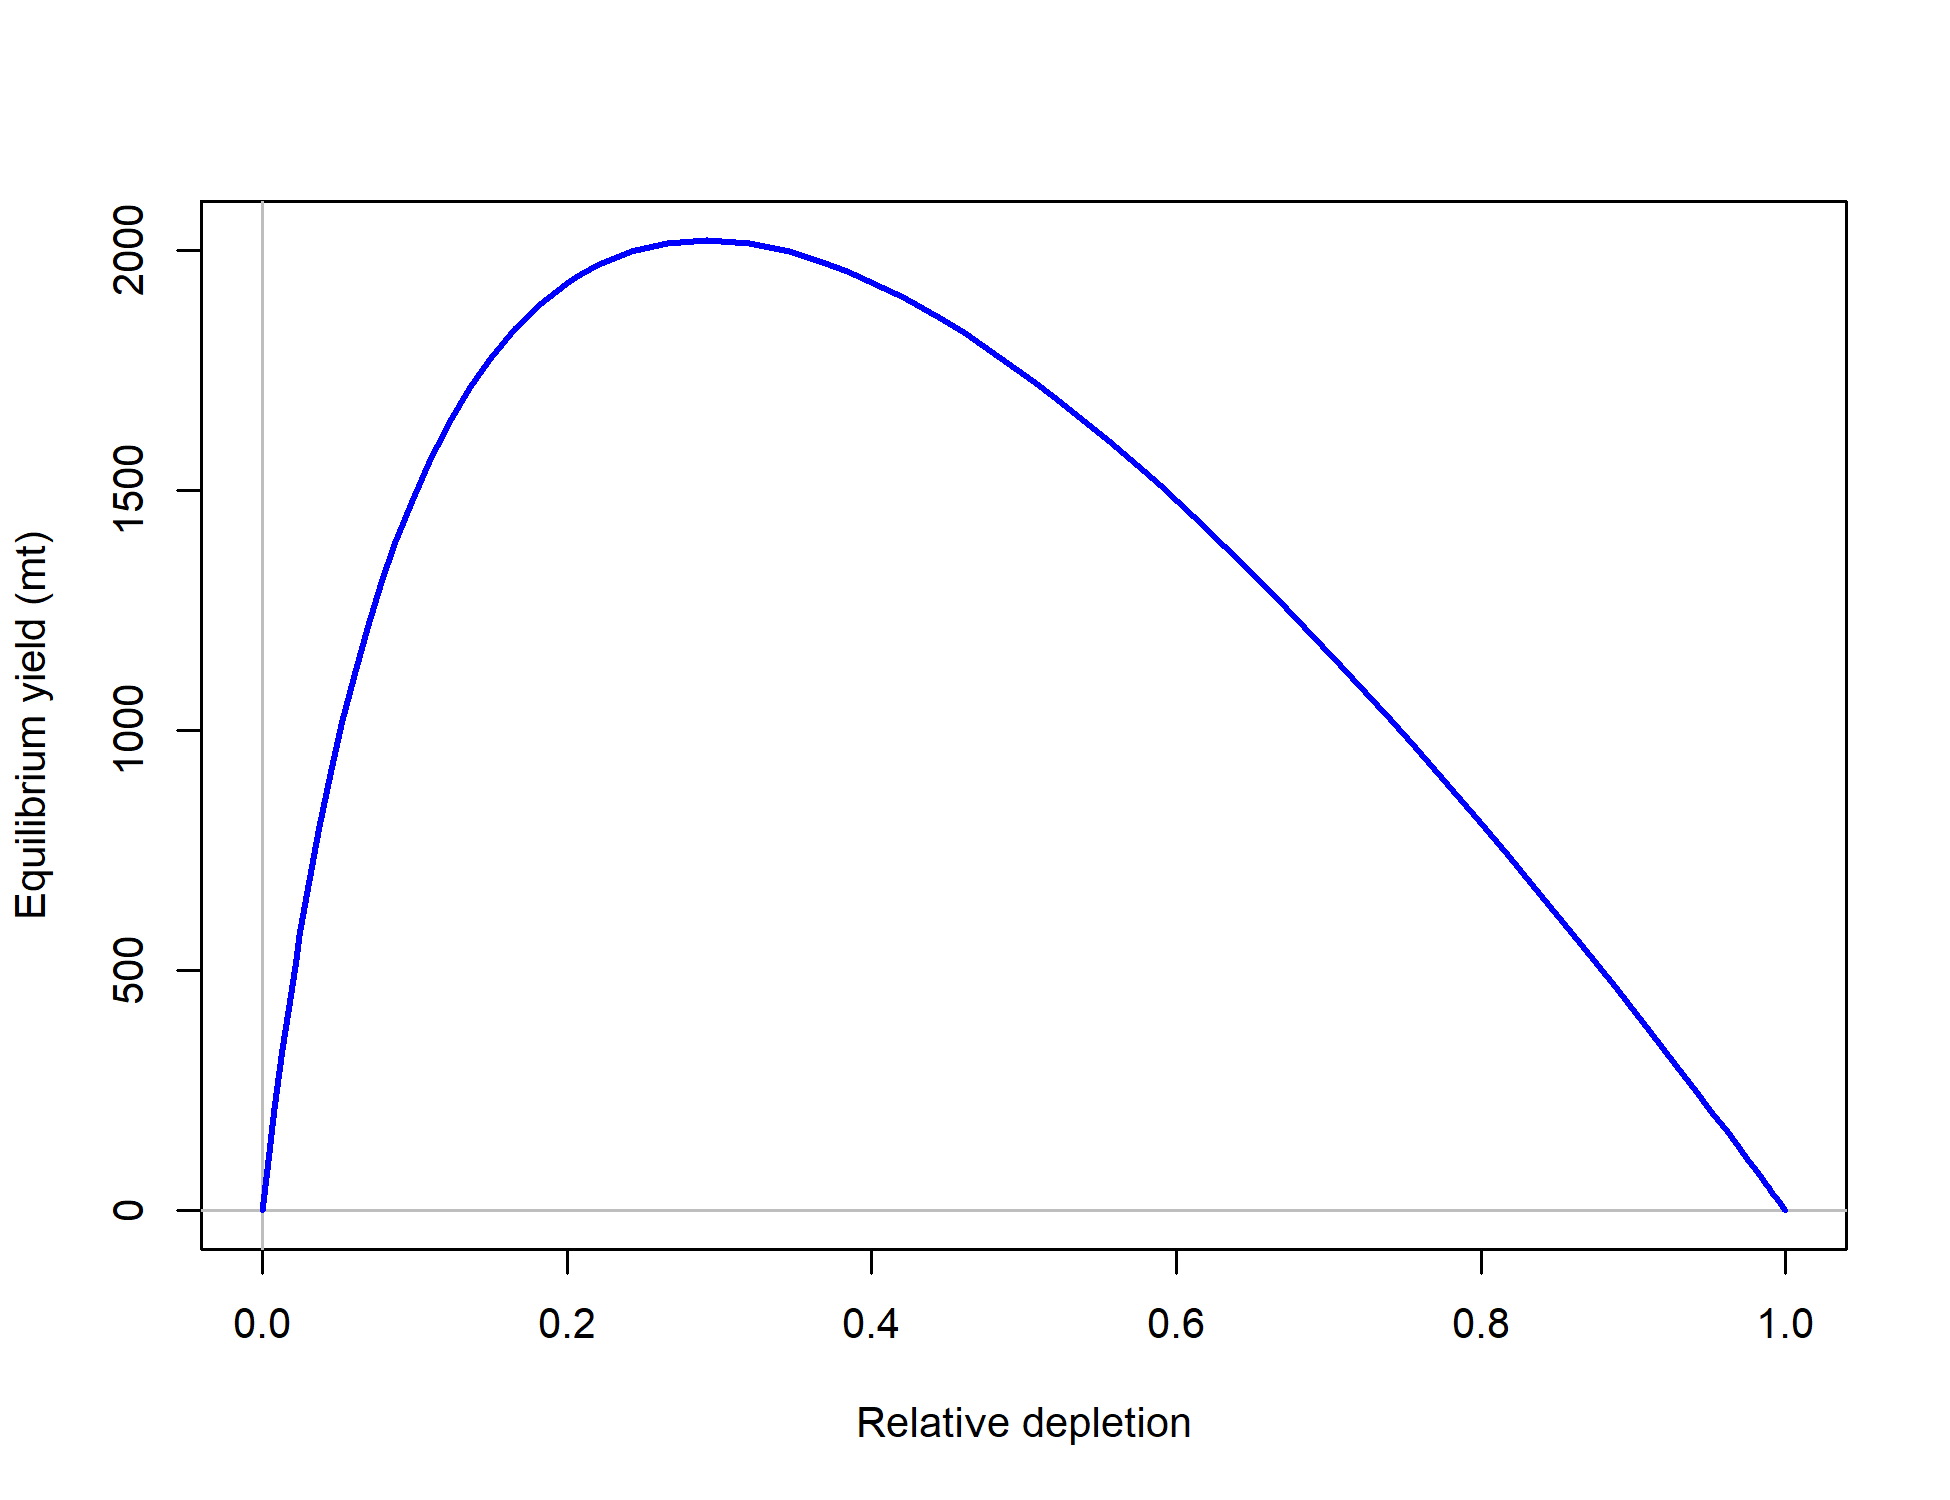
\includegraphics{r4ss/plots_mod1/yield1_yield_curve.png}
\caption{Equilibrium yield curve for the base case model. Values are
based on the 2014 fishery selectivity and with steepness fixed at 0.718.
\label{fig:Yield_all}}
\end{figure}

\FloatBarrier

\newpage

\section*{Executive summary for the Oregon
Model}\label{executive-summary-for-the-oregon-model}
\addcontentsline{toc}{section}{Executive summary for the Oregon Model}

\FloatBarrier

\begin{figure}[htbp]
\centering
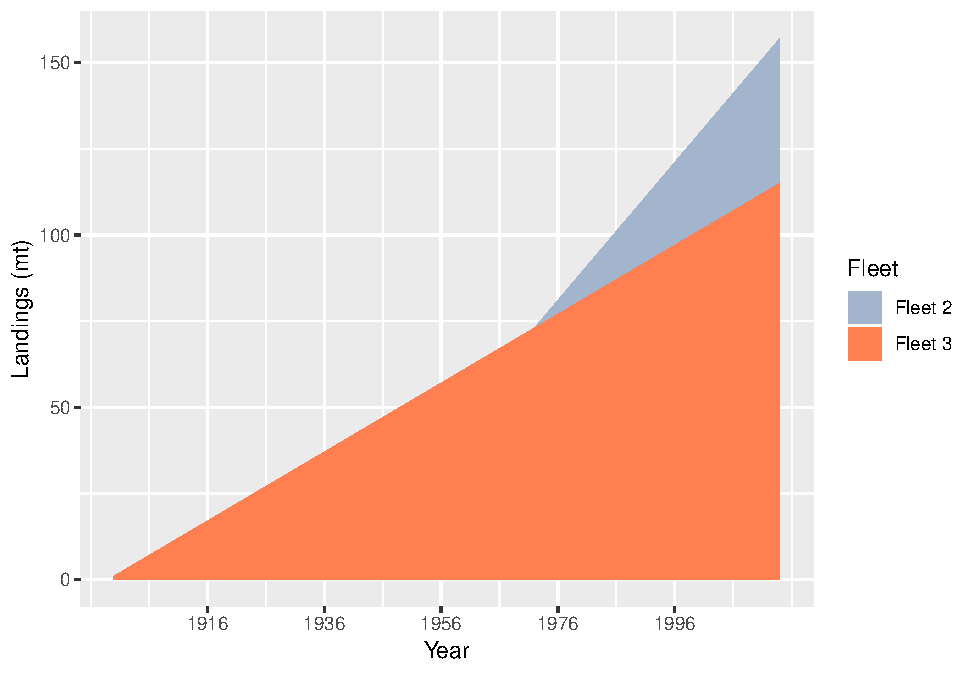
\includegraphics{00_Assessment_Compile_files/figure-latex/unnamed-chunk-13-1.pdf}
\caption{Stacked line plot of Black Rockfish catch history for the
commercial fleets. \label{fig:Exec_catch2}}
\end{figure}

\FloatBarrier

\begin{figure}[htbp]
\centering
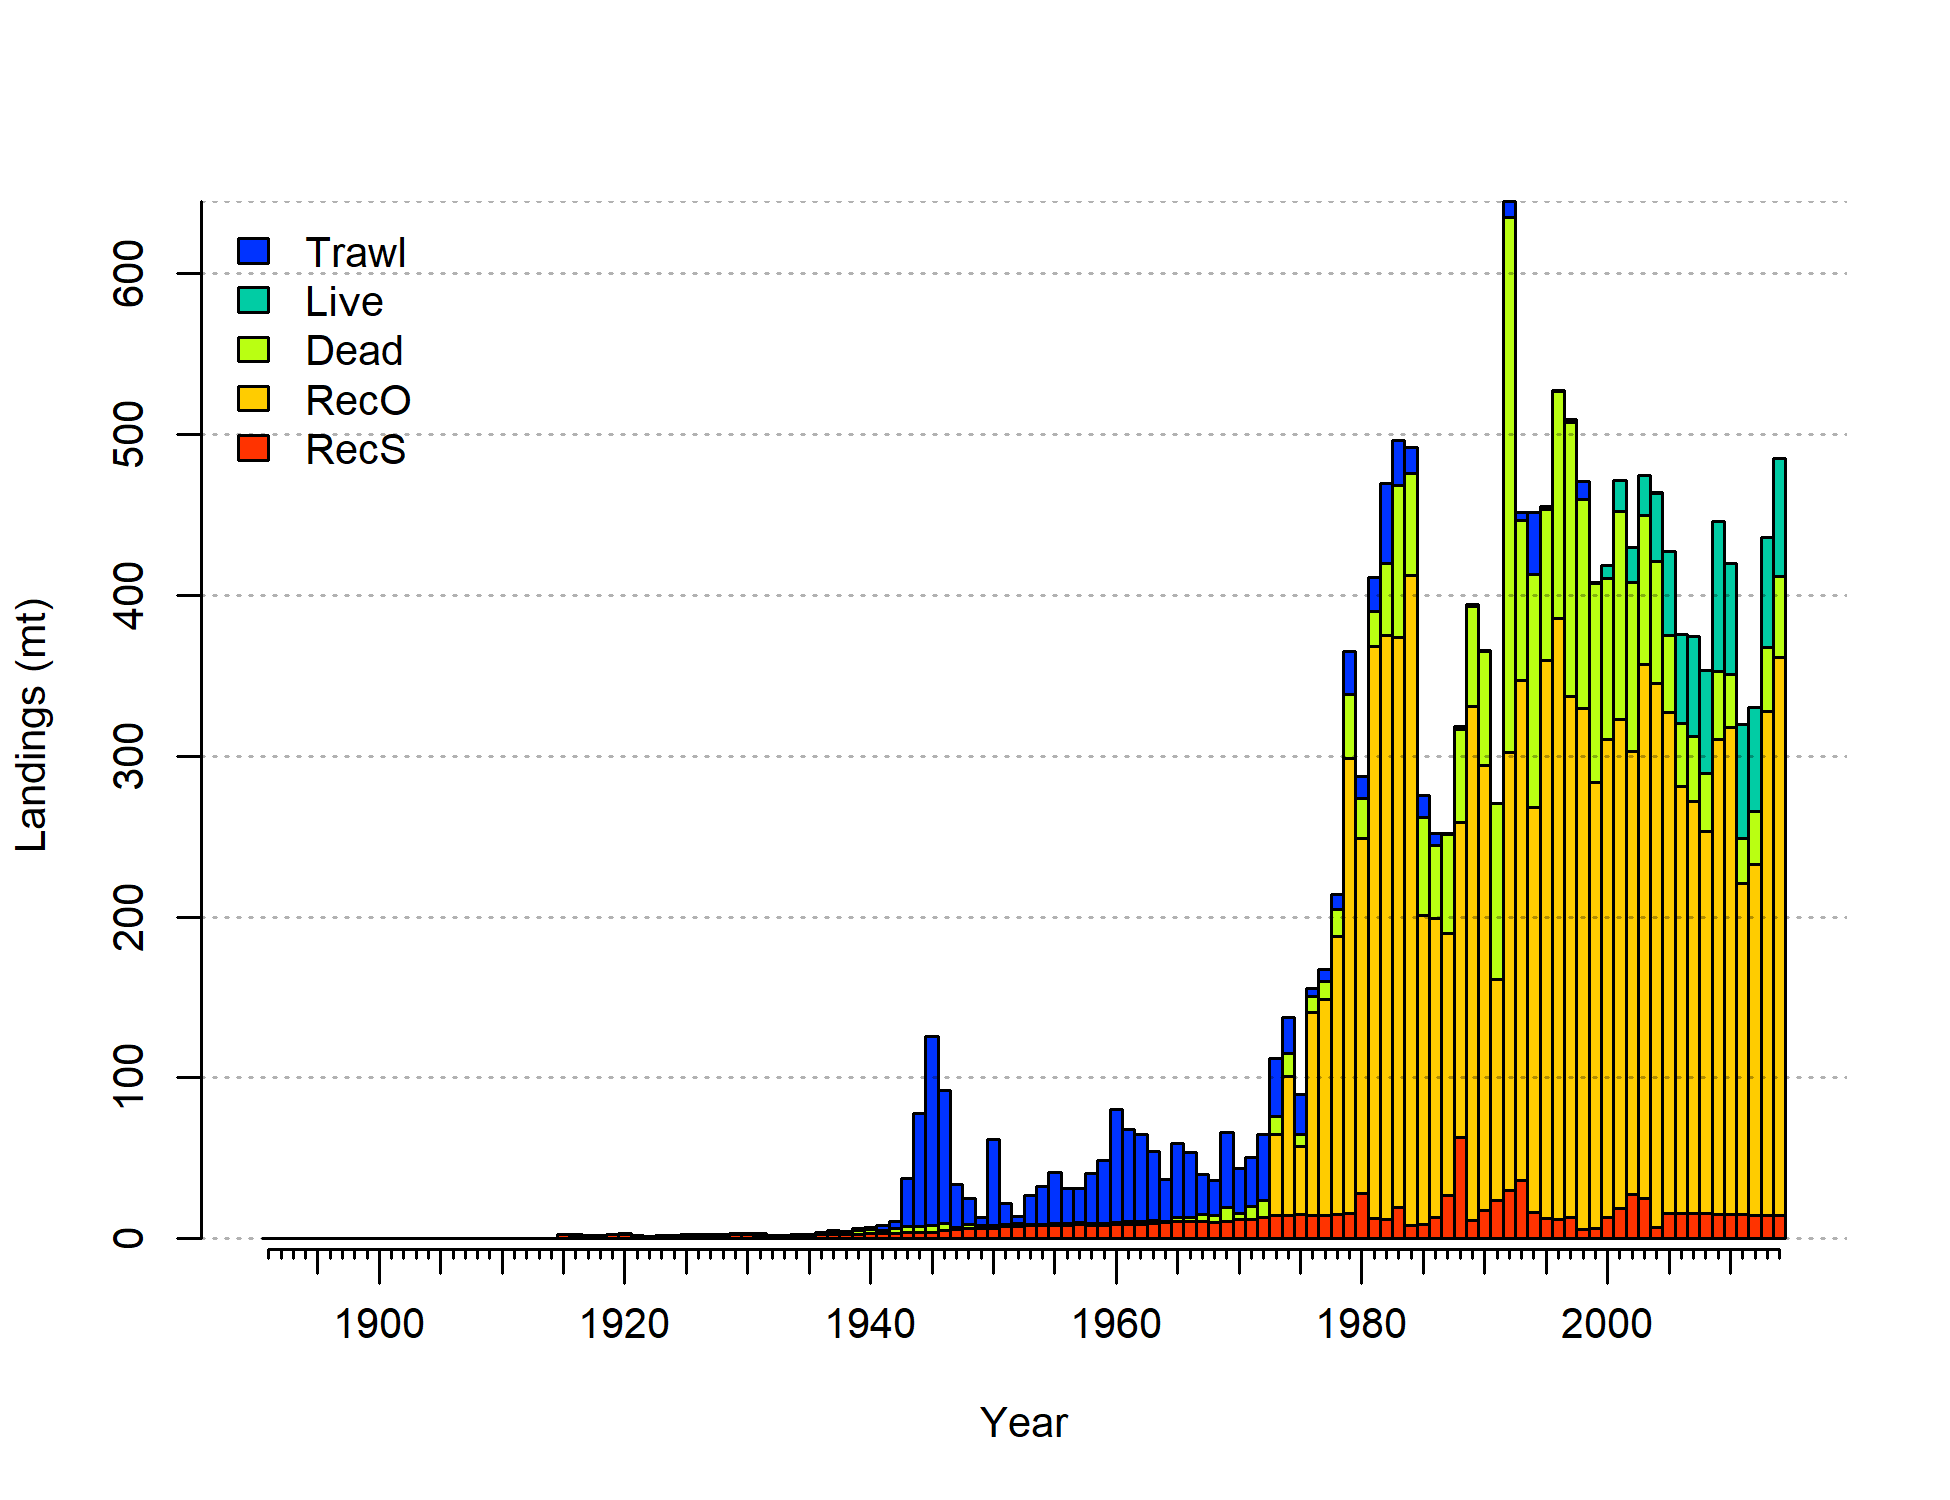
\includegraphics{r4ss/plots_mod2/catch2 landings stacked.png}
\caption{Catch history of Black Rockfish in the California model.
\label{fig:r4ss_catches2}}
\end{figure}

\begin{table}[ht]
\centering
\caption{Recent Black Rockfish landings (mt) by 
                                            fleet.} 
\label{tab:Exec_catch}
\begin{tabular}{l>{\centering}p{1in}>{\centering}p{1in}>{\centering}p{1in}>{\centering}p{.9in}>{\centering}p{.9in}>{\centering}p{.6in}}
  \hline
Year & Landings 1 & Landings 2 & Landings 3 & Landings 4 & Landings 5 & Total \\ 
  \hline
2005 & - & - & - & - & - & - \\ 
  2006 & - & - & - & - & - & - \\ 
  2007 & - & - & - & - & - & - \\ 
  2008 & - & - & - & - & - & - \\ 
  2009 & - & - & - & - & - & - \\ 
  2010 & - & - & - & - & - & - \\ 
  2011 & - & - & - & - & - & - \\ 
  2012 & - & - & - & - & - & - \\ 
  2013 & - & - & - & - & - & - \\ 
  2014 & - & - & - & - & - & - \\ 
   \hline
\end{tabular}
\end{table}

\FloatBarrier

\newpage

\subsection*{Stock Biomass}\label{stock-biomass-1}
\addcontentsline{toc}{subsection}{Stock Biomass}

(Figure \ref{fig:Spawnbio_all2} and Table
\ref{tab:SpawningDeplete_mod2}).

The 2014 estimated spawning biomass relative to unfished equilibrium
spawning biomass is above the target of 40\% of unfished spawning
biomass at 60.3\% (95\% asymptotic interval: \(\pm\) 18.9\%-47.7\%)
(Figure \ref{fig:RelDeplete_all}). Approximate confidence intervals
based on the asymptotic variance estimates show that the uncertainty in
the estimated spawning biomass is high.

\FloatBarrier

\begin{table}[ht]
\centering
\caption{Recent trend in 
                                             beginning of the year spawning output
                                             and depletion for the Oregon model for Black Rockfish.} 
\label{tab:SpawningDeplete_mod2}
\begin{tabular}{l>{\centering}p{1.3in}>{\centering}p{1.2in}>{\centering}p{1in}>{\centering}p{1.2in}}
  \hline
Year & Spawning Output (million eggs) & \~{} 95\% confidence interval & Estimated depletion & \~{} 95\% confidence interval \\ 
  \hline
2006 & 776.596 & (676.31-876.88) & 0.589 & (0.575-0.604) \\ 
  2007 & 778.375 & (678.43-878.32) & 0.590 & (0.576-0.605) \\ 
  2008 & 781.352 & (681.55-881.15) & 0.593 & (0.578-0.607) \\ 
  2009 & 786.954 & (687.07-886.84) & 0.597 & (0.583-0.611) \\ 
  2010 & 785.401 & (685.38-885.42) & 0.596 & (0.582-0.61) \\ 
  2011 & 785.753 & (685.59-885.92) & 0.596 & (0.582-0.61) \\ 
  2012 & 793.377 & (692.97-893.79) & 0.602 & (0.588-0.616) \\ 
  2013 & 800.964 & (700.14-901.79) & 0.608 & (0.594-0.621) \\ 
  2014 & 800.461 & (699.23-901.69) & 0.607 & (0.593-0.621) \\ 
  2015 & 794.603 & (693.2-896.01) & 0.603 & (0.588-0.617) \\ 
   \hline
\end{tabular}
\end{table}

\FloatBarrier

--\textgreater{}

--\textgreater{}

--\textgreater{}

--\textgreater{}

--\textgreater{} --\textgreater{}

--\textgreater{} --\textgreater{}

--\textgreater{}

--\textgreater{}

--\textgreater{} --\textgreater{}

--\textgreater{}

--\textgreater{}

--\textgreater{}

\section*{Executive summary for the Washington
Model}\label{executive-summary-for-the-washington-model}
\addcontentsline{toc}{section}{Executive summary for the Washington
Model}

\FloatBarrier

\begin{figure}[htbp]
\centering
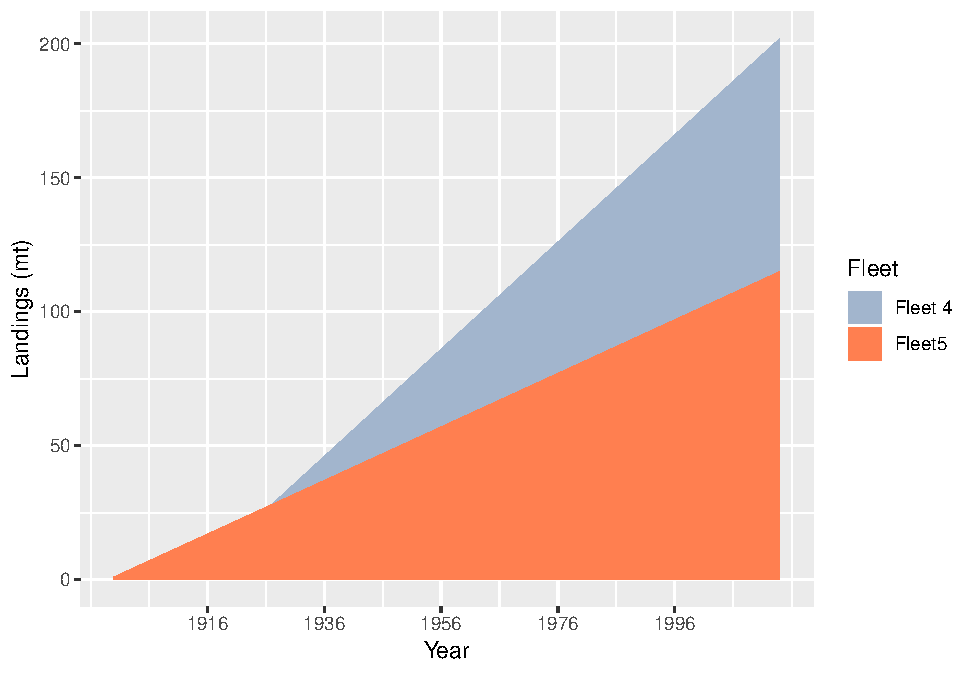
\includegraphics{00_Assessment_Compile_files/figure-latex/unnamed-chunk-16-1.pdf}
\caption{Black Rockfish catch history for the recreational fleets.
\label{fig:Exec_catch3}}
\end{figure}

\FloatBarrier

\begin{figure}[htbp]
\centering
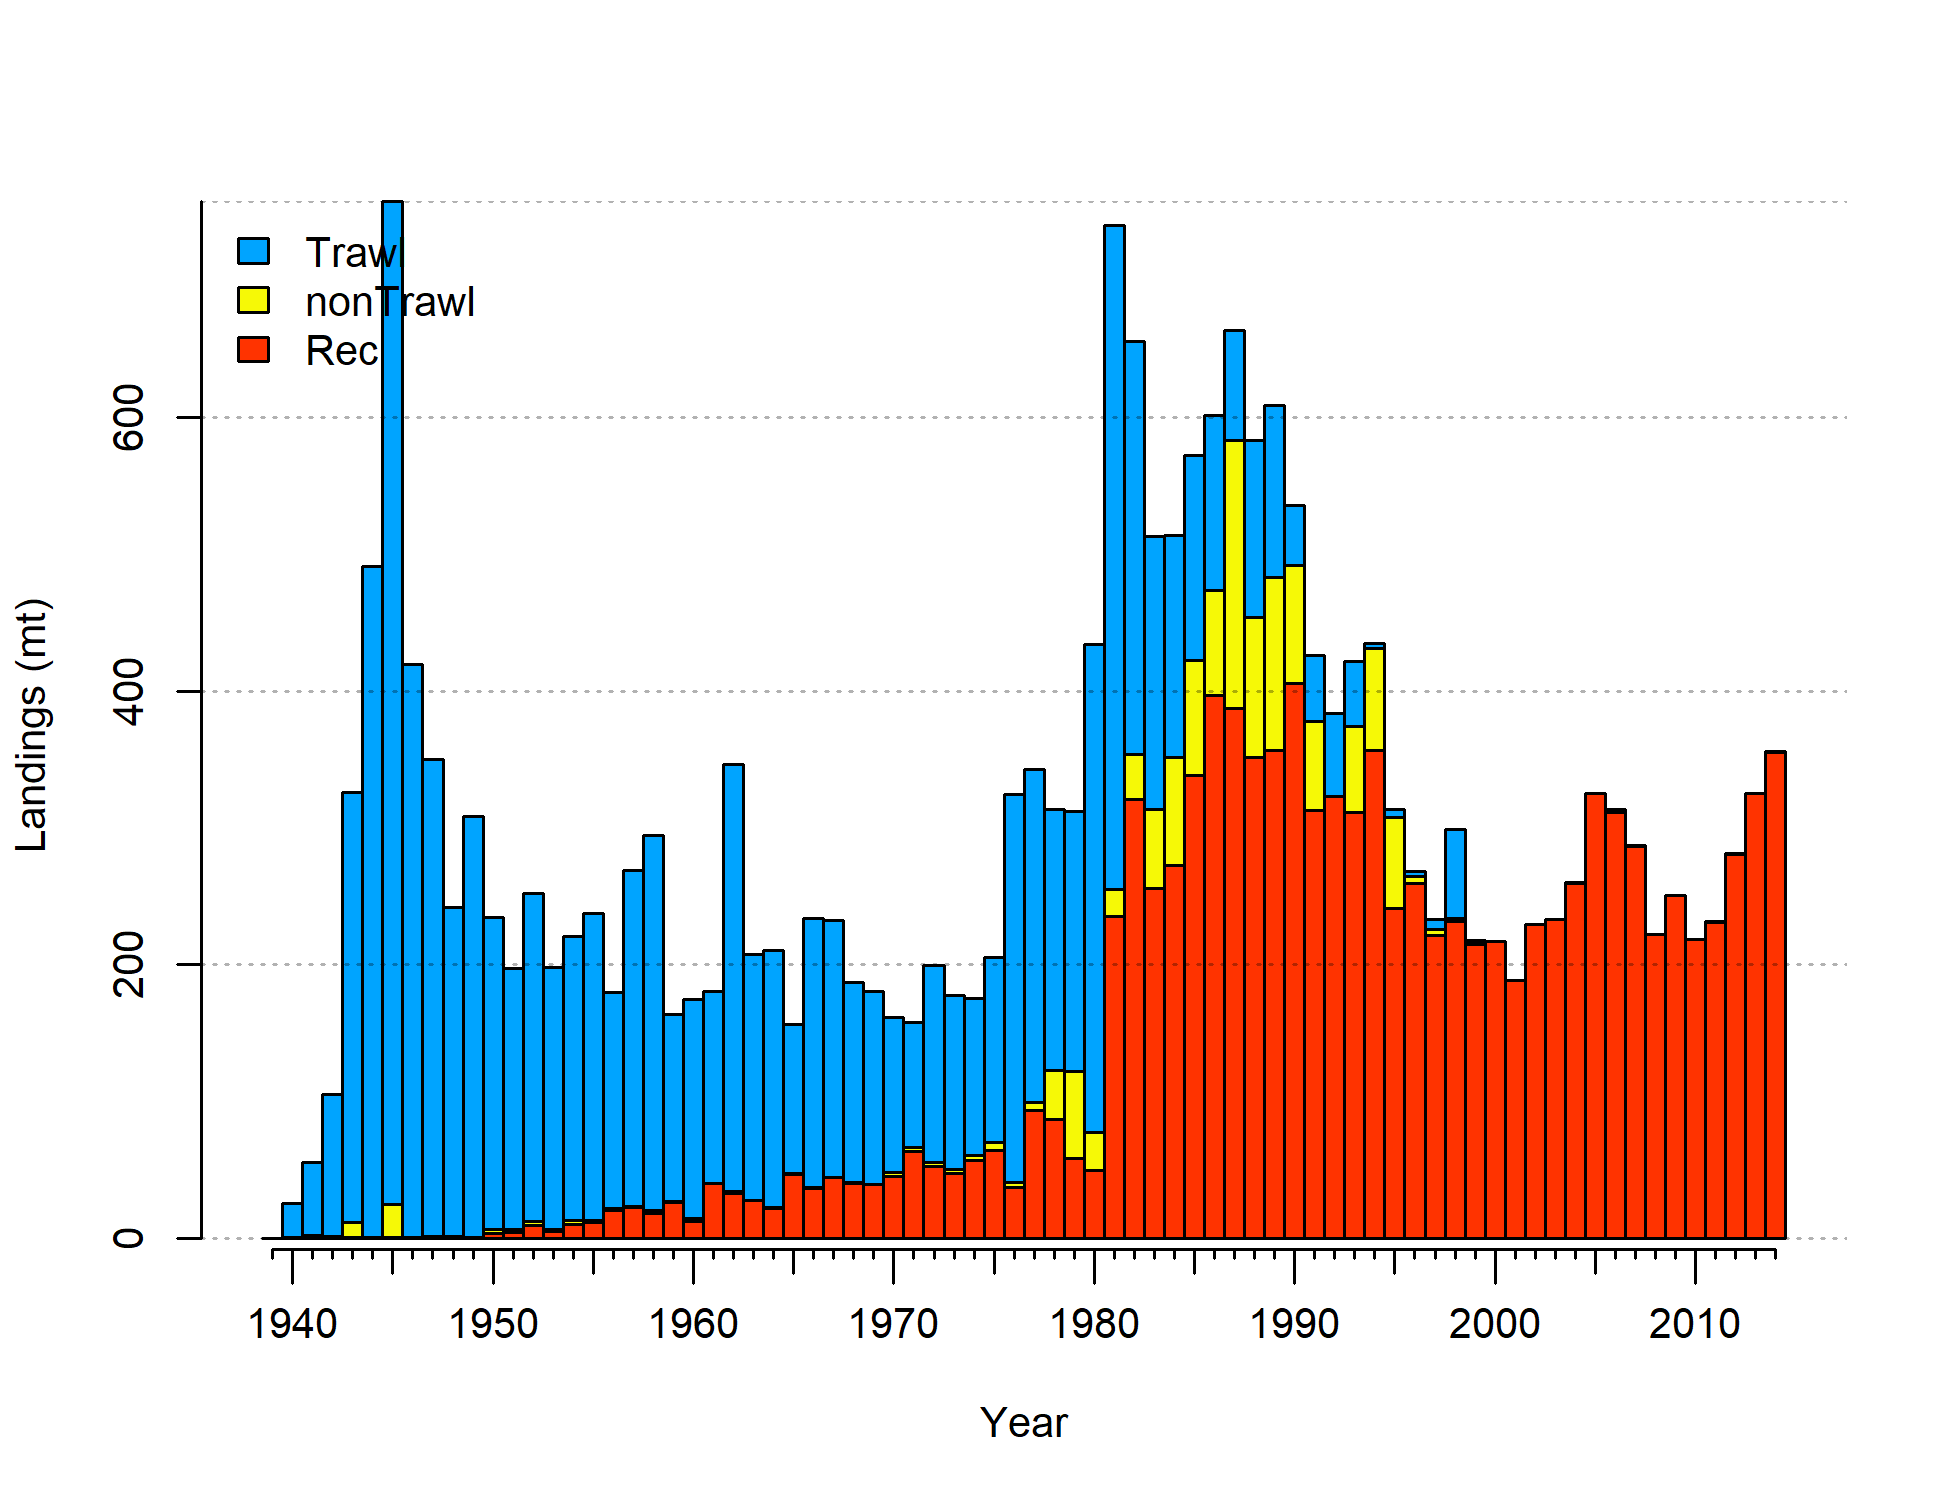
\includegraphics{r4ss/plots_mod3/catch2 landings stacked.png}
\caption{Catch history of Black Rockfish in the Washington model.
\label{fig:r4ss_catches3}}
\end{figure}

\begin{table}[ht]
\centering
\caption{Recent Black Rockfish landings (mt) by 
                                            fleet.} 
\label{tab:Exec_catch}
\begin{tabular}{l>{\centering}p{1in}>{\centering}p{1in}>{\centering}p{1in}>{\centering}p{.9in}>{\centering}p{.9in}>{\centering}p{.6in}}
  \hline
Year & Landings 1 & Landings 2 & Landings 3 & Landings 4 & Landings 5 & Total \\ 
  \hline
2005 & - & - & - & - & - & - \\ 
  2006 & - & - & - & - & - & - \\ 
  2007 & - & - & - & - & - & - \\ 
  2008 & - & - & - & - & - & - \\ 
  2009 & - & - & - & - & - & - \\ 
  2010 & - & - & - & - & - & - \\ 
  2011 & - & - & - & - & - & - \\ 
  2012 & - & - & - & - & - & - \\ 
  2013 & - & - & - & - & - & - \\ 
  2014 & - & - & - & - & - & - \\ 
   \hline
\end{tabular}
\end{table}

\FloatBarrier

\newpage

--\textgreater{}

--\textgreater{}

--\textgreater{}

--\textgreater{}

--\textgreater{}

--\textgreater{} --\textgreater{}

--\textgreater{} --\textgreater{}

--\textgreater{}

--\textgreater{}

--\textgreater{} --\textgreater{}

--\textgreater{}

--\textgreater{}

--\textgreater{}

--\textgreater{}

--\textgreater{}

\newpage

\color{black}

\section*{References}\label{references}
\addcontentsline{toc}{section}{References}

\renewcommand{\thepage}{}

\end{document}
